\documentclass[11pt,final,oneside]{fithesis}
\usepackage[plainpages=false, pdfpagelabels]{hyperref}
\usepackage{amssymb}
\usepackage{amsmath}
\usepackage{graphicx}
\usepackage{wrapfig}
\usepackage[T1]{fontenc}
\usepackage[latin2]{inputenc}
\usepackage[slovak]{babel}

\graphicspath{{images/}}
%\bibliographystyle{plain}

\thesislang{sk}
\thesistitle{Roz\v s\'irenie a refaktoriz\'acia n\'astroja BioDiVinE}
\thesissubtitle{Diplomov\' a pr\' aca}
\thesisstudent{Martin Demko}
\thesiswoman{false}
\thesisfaculty{fi}
\thesisyear{jar 2014}
\thesisadvisor{RNDr. David \v Safr\' anek, Ph.D.}

\begin{document}
\FrontMatter
\ThesisTitlePage


\begin{ThesisDeclaration}
\DeclarationText
\AdvisorName
\end{ThesisDeclaration}

\begin{ThesisThanks}
\end{ThesisThanks}

\begin{ThesisAbstract}
\end{ThesisAbstract}

\begin{ThesisKeyWords}
\end{ThesisKeyWords}

%====================================OBSAH==================================================
\MainMatter
\tableofcontents
%====================================UVOD===================================================
\chapter*{\' Uvod}

%================================ZAKLADNE=POJMY=============================================
\chapter{Z\' akladn\' e pojmy}
Ne\v z za\v cneme zach\' adza\v t hlb\v sie do problematiky tejto pr\' ace a opisova\v t postupy a n\' astroje v nej pou\v zit\' e, 
je potrebn\' e vysvetli\v t na po\v ciatku nieko\v lko pojmov. Tieto sa v pr\' aci mnohokr\' at opakuj\' u a ich v\v casn\' ym uveden\' im
pred\' ideme nepochopite\v lnosti textu. Je tie\v z d\^ ole\v zit\'e poznamena\v t, \v ze t\'ato kapitola je z ve\v lkej miery doslovne citovan\'a
zo zdrojov uveden\'ych v\v zdy na konci ka\v zdej podkapitoly.

%-------------------------------------------------------------------------------------------
\section{LTL - Line\' arna Tempor\' alna Logika}
\label{sec:logika}
Tempor\' alna logika obecne je \v speci\' alna vetva logiky zaoberaj\' uca sa logickou \v strukt\' urou v\' yrokov v \v case. 
Je to formalizmus vhodn\' y pre overovanie vlastnost\' i form\' alnych dynamick\' ych syst\' emov resp. matematick\' ych modelov.

Line\' arna tempor\' alna logika (\v dalej len LTL) je najjednoduch\v sia verzia tempor\' alnej logiky, ktor\' a neumo\v z\v nuje vetvenie \v casu 
ani kvantifik\' atory.
M\^ o\v zeme ju pova\v zova\v t tie\v z za konkr\' etny v\' ypo\v ctov\' y kalkulus pracuj\' uci s tzv. formulami, definovan\' ymi nasleduj\' ucou syntaxou:
\begin{description}
\item[Atomick\' e propoz\' icie] (\v dalej len $AP$) \hfill
\begin{center}
$A > 0$ \\
$B \leq 5.834$ \\
$C \neq "nie"$ \\
{\it at\v d$\dots{}$}
\end{center}
\item[Logick\' e oper\' atory] \hfill
\begin{align*}
&\neg, \ \vee &-& \ \textrm{\it z\' akladn\' e logick\' e oper\' atory}\\
&\wedge , \ \rightarrow , \ \leftrightarrow , \ \mathbf{true} , \ \mathbf{false} \hfil &-& \ \textrm{\it odvoden\' e logick\' e oper\' atory}
\end{align*}
\item[Tempor\' alne oper\' atory] \hfill
\begin{itemize}
\item $\mathbf{X} \phi$ \ - \ \textrm{ne}$\mathbf{X}$\textrm{t, {\it vyjadruje platnos\v t $\phi$ v \v dal\v som stave}}
\item $\mathbf{G} \phi$ \ - \ $\mathbf{G}$\textrm{lobal, {\it vyjadruje trval\' u platnos\v t $\phi$ }}
\item {$\mathbf{F} \phi$} \ - \ $\mathbf{F}$\textrm{uture, {\it vyjadruje platnos\v t $\phi$ v niektorom z bud\' ucich stavov }}
\item {$\psi \mathbf{U} \phi$} \ - \ $\mathbf{U}$\textrm{ntil, {\it vyjadruje platnos\v t $\psi$ a\v z do kedy neza\v cne plati\v t $\phi$}}
\item {$\psi \mathbf{R} \phi$} \ - \ $\mathbf{R}$\textrm{elease, {\it vyjadruje platnos\v t $\phi$, a\v z dokedy neza\v cne plati\v t $\psi$ 
a to vr\'atane tohto bodu. Ak $\psi$ nikdy neza\v cne plati\v t, mus\'i $\phi$ plati\v t do nekone\v cna}}\\
\\
{\it kde $\phi$ a $\psi$ s\' u atomick\' e propoz\' icie}
\end{itemize}
\end{description}
Potom plat\'i nasleduj\'uce:
\begin{itemize}
\item Ak $p \in AP$, tak $p$ je formula.
\item Ak $f$ a $g$ s\'u formule, tak $\neg g$, $f \lor g$, $f \wedge g$, $f \rightarrow g$, $f \leftrightarrow g$, $\mathbf{X} g$, $\mathbf{F} g$, 
$\mathbf{G} g$, $f \mathbf{U} g$ a $g \mathbf{R} f$ s\'u formule.
\end{itemize}
Takto vytvoren\'a LTL formula m\^ o\v ze by\v t splnite\v ln\'a nekone\v cnou postupnos\v tou pravdiv\'ych vyhodnoten\'i jednotliv\'ych $p \in AP$. 
T\'uto postupnos\v t si mo\v zno predstavi\v t ako nekone\v cn\'e slovo $w$, pre ktor\'e plat\'i $w = a_0,a_1,a_2,\dots{}$ a kde $a_i$ je pravdivostn\'a hodnota
nejakej $p \in AP$. Nech $w(i) = a_i$ a $w^i = a_i,a_{i+1},\dots{}$ je podpostupnos\v t alebo sufix slova $w$. Potom form\'alna defin\'icia rel\'acie splnite\v lnosti
$\vDash$ medzi slovom $w$ a LTL formulov vyzer\'a:
\begin{itemize}
\item $w \vDash p$,\hfil ak $p \in AP$ $\bigwedge$ $p = w(0)$
\item $w \vDash \neg\phi$,\hfil ak $\phi$ a $\psi$ s\'u LTL formule $\bigwedge$ $w \nvDash \phi$
\item $w \vDash \phi \vee \psi$,\hfil ak $w \vDash \phi$ $\bigvee$ $w \vDash \psi$
\item $w \vDash {\bf X}\phi$,\hfil ak $w^1 \vDash \phi$
\item $w \vDash \phi {\bf U} \psi$,\hfil ak $\exists i,\ i \geq 0 \wedge w^i \vDash \psi$ $\bigwedge$ $\forall k,\ 0 \leq k < i \wedge w^k \vDash \phi$
\end{itemize}
Predch\'adzaj\'uce plat\'i pre z\'akladn\'e logick\'e a tempor\'alne oper\'atory, ktor\'e maj\'u ale dostato\v cne expres\'ivnu silu, aby s ich pomocou
mohli by\v t zadefinovan\'e \v lubovoln\'e LTL formule. Ov\v sem pre u\v lah\v cenie z\'apisu aj \v c\'itania, si m\^ o\v zeme dodefinova\v t roz\v s\'iren\'u
paletu oper\'atorov za predpokladu platnosti predch\'adzaj\'ucich pravidiel:
\begin{itemize}
\item $\phi \wedge \psi \ \equiv \ \neg(\neg \phi \vee \neg \psi)$,\hfil ak $\phi, \psi$ s\'u LTL formule
\item $\phi \rightarrow \psi \ \equiv \ \neg \psi \vee \psi$,
\item $\phi \leftrightarrow \psi \ \equiv \ (\phi \rightarrow \psi) \vee (\psi \rightarrow \phi)$,
\item $\mathbf{true} \ \equiv \ p \vee \neg p$,\hfil ak $p \in AP$
\item $\mathbf{false} \ \equiv \ \neg\mathbf{true}$,
\item $\phi {\bf R} \psi \ \equiv \ \neg(\neg\phi{\bf U}\neg\psi)$,
\item $\mathbf{F} \phi \ \equiv \ \mathbf{true U} \phi$,
\item $\mathbf{G} \phi \ \equiv \ \neg \mathbf{F} \neg \phi$,
\end{itemize}
Napriek tomu, \v ze je LTL tou najprimit\' ivnej\v sou tempor\'alnou logikou, jej prevod do B\"uchiho automatu je v najhor\v som pr\' ipade 
exponenci\' alne zlo\v zit\' y. D\^ ovod tohto prevodu bude vysvetlen\' y v kapitole \ref{sec:modelChecking}. 
\cite{Clarke:MC:LTL}

%-------------------------------------------------------------------------------------------
\section{B\"uchiho automat}	%kniha Model checking str. 121
\label{sec:buchi}
Automat obecne je matematick\' y model stroja s kone\v cn\' ym mno\v zstvom pam\" ate spracov\' avaj\' uci vstup o nezn\' amej ve\v lkosti. 
Kv\^ oli obmedzeniu pam\" ate ho naz\' yvame kone\v cn\' ym automatom. Vstup sa naz\' yva slovo a m\^ o\v ze by\v t kone\v cn\' y aj nekone\v cn\' y.
B\" uchiho automat je potom najjednoduch\v s\' im kone\v cn\'ym automatom nad nekone\v cn\'ym slovom a preto patr\'i do skupiny {$\omega$"~au\-to\-matov}.

Form\'alne je kone\v cn\' y automat $\mathcal{A}$ p\" atica $(\Sigma, Q, \Delta, Q_0, F)$, pre ktor\' u plat\'i:
\begin{itemize}
\item $\Sigma$\ je kone\v cn\'a abeceda
\item $Q$\ je kone\v cn\'a mno\v zina stavov
\item $\Delta \subseteq Q \times \Sigma \times Q$\ je rel\' acia naz\'yvan\'a prechodov\'a funkcia
\item $Q_0 \subseteq Q$ je podmno\v zina mno\v ziny stavov, naz\' yvan\' a inici\' alne stavy
\item $F \subseteq Q$ je podmno\v zina mno\v ziny stavov, naz\'yvan\'a akceptuj\'uce stavy
\end{itemize}
Pr\'iklad jednoduch\'eho automatu je dan\'y na obr\'azku \ref{fig:buchi}.

Automat nad kone\v cn\'ym slovom akceptuje toto slovo, ak po prejden\' i poslen\'eho znaku slova zodpovedaj\' uceho prechodu medzi dvoma stavami, 
je tento posledn\' y stav v mno\v zine $F$. Av\v sak automat nad nekone\v cn\' ym slovom nem\^ o\v ze nikdy prejs\v t cez posledn\' y znak. Preto tak\' yto 
automat akceptuje nekone\v cn\' e slovo len v pr\' ipade, \v ze po\v cas prech\' adzania slova je aspo\v n jeden stav nav\v st\'iven\'y nekone\v cne \v casto 
a z\'arove\v n tento stav patr\'i aj do mno\v ziny $F$.

Automaty m\^ o\v zeme e\v ste rozl\'i\v si\v t na deterministick\'e a nedeterministick\'e. Deterministick\' y automat m\'a jednozna\v cne ur\v cen\'e prechody 
medzi stavmi. T\'ym sa mysl\'i, \v ze zo stavu $q \in Q$ sa pod znakom $s \in \Sigma$ d\'a prejs\v t maxim\'alne do jednoho stavu $q^{'} \in Q$. Naproti tomu
nedeterministick\'e automaty umo\v z\v nuj\'u prechod zo stavu $q$ pod slovom $s$ do stavov $Q^{'} \subseteq Q$. Na\v s\v tastie existuje algoritmus prevodu 
nedeterministick\'eho kone\v cn\'eho automatu  na deterministick\'y, ale iba nad kone\v cn\'ym slovom. Nev\'yhodou je ale ve\'lk\'y n\'arast po\v ctu stavov.
\cite{Clarke:MC:BA}
\begin{figure}[h]
	\centering
	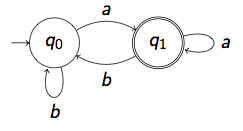
\includegraphics[width=0.4\textwidth]{buchi1}
	\caption{Jednoduch\'y deterministick\'y automat $\mathcal{A} :$ $\Sigma = \{a,b\},$ $Q = \{q_0,q_1\},$ $\Delta = \{(q_0,a,q_1),(q_0,b,q_0),(q_1,a,q_1),(q_1,b,q_0)\},$ 
	$Q_0 = \{q_0\}$, $F = \{q_1\}$}
	\label{fig:buchi}
\end{figure}

%-------------------------------------------------------------------------------------------
\section{Z\'akon o mass action kinetike}
\label{sec:massAction}
Tento z\'akon vyjadruje z\'akladn\'e pravidlo fungovania chemick\'ych reakci\'i. Konkr\'etne r\'ychlos\v t s akou chemick\'e substancie, \v ci u\v z 
ve\v lk\'e makromolekuly alebo mal\'e i\'ony, do seba nar\'a\v zaj\'u a interaguj\'u za tvorby nov\'ych chemick\'ych l\'atok. Predpokladajme, \v ze
substr\'aty $A$ a $B$ spolu reaguj\'u za vzniku novej l\'atky, produktu $C$,
\begin{equation}
\label{eq:simpleReaction}
A + B \overset{k}{\longrightarrow} C.
\end{equation}

R\'ychlos\v t tejto reakcie predstavuje r\'ychlos\v t tvorby produktu $C$, a s\'ice $\frac{d[C]}{dt}$, ktor\'a steles\v nuje po\v cet kol\'izi\'i za jednotku 
\v casu medzi reaktantami $A$ a $B$ a z\'arove\v n pravdepodobnos\v t, \v ze tieto kol\'izie maj\'u dostato\v cn\'u energiu na prekonannie aktiva\v cnej 
energie reakcie. To samozrejme z\'ale\v z\'i po prv\'e na koncentr\'acii reaktantov, ale aj na ich tvare a ve\v lkosti a tie\v z na teplote a ph roztoku. 
Kombin\'aciou t\'ychto a aj \v dal\v s\'ich faktorov dost\'avame neline\'arnu ordin\'arnu diferenci\'alnu rovnicu (z \textit{ang.} ordinary differential 
equation, skr\'atene ODE) \cite{ODE}:
\begin{equation}
\label{eq:differentialReaction}
\frac{d[C]}{dt} = k[A][B]
\end{equation}

Identifik\'acia vz\v tahu \ref{eq:simpleReaction} s rovnicou \ref{eq:differentialReaction} sa naz\'yva z\'akon mass action kinetiky (z \textit{ang.} law of mass action) a kon\v stanta $k$ 
je potom r\'ychlostn\'a kon\v stanta (z \textit{ang.} rate constant) tejto reakcie.

V skuto\v cnosti nejde o z\'akon ako tak\'y. Nie je to neporu\v site\v ln\'e pravidlo ako Newtonov gravita\v cn\'y z\'akon, ale sk\^ or ve\v lmi 
u\v zito\v cn\'y model, ktor\'y v\v sak nemus\'i by\v t vo v\v setk\'ych pr\'ipadoch validn\'y. \cite{Keener:1998:MP:MassAction}

%-------------------------------------------------------------------------------------------
\section{Michaelis-Mentenovej a Hillova kinetika}
\label{kinetiky}
%[odkaz na wiki a LectureNotes.pdf]
Je nutn\'e za\v ca\v t od enz\'ymovej kinetiky, preto\v ze pr\'ave t\'a bola hlavn\'ym kataly\-z\'atorom pre objavenie nov\'ych sp\^ osobov modelovania 
chemick\'ych reakci\'i. Tie\v z je dobr\'e si uvedomi\v t, pre\v co tomu tak bolo. Enz\'ymov\'a kinetika toti\v z patr\'i medzi nieko\v lko pr\'ipadov, 
v ktor\'ych pou\v zitie mass action kinetiky nie je validn\'e. Pod\v la nej sa so zvy\v zuj\'ucou koncentr\'aciou substr\'atu $S$ zvy\v suje r\'ychlos\v t
reakcie zlu\v covania s enz\'ymom $E$ line\'arne. Zatia\v l \v co v \textit{in-vivo} pr\'ipade t\'ato r\'ychlos\v t postupne konverguje k ur\v cit\'emu 
maximu, cez ktor\'e sa ned\'a dosta\v t ani dodato\v cn\'ym zv\'y\v sen\'im koncentr\'acie substr\'atu $S$.

Model, ktor\'y vysvet\v loval t\'uto odch\'ylku od z\'akona o mass action kinetike bol prv\'y kr\'at prezentovan\'y v roku 1913 nemeck\'ym biochemikom Leonardom 
Michaelisom a kanadskou fyzi\v ckou Maud Mentenovou (z toho \textit{kinetika Michaelis-Mentenovej}). V ich reakcii premie\v nal enz\'ym $E$ subtr\'at $S$ 
na produkt $P$ v dvoch f\'azach. Prv\'a bola reverzibiln\'a reakcia zlu\v covania $S$ s~$E$ za vzniku enz\'ym"~substr\'atov\'eho komplexu $C$ a druh\'a 
predstavovala rozpad komplexu $C$ za vzniku produktu $P$ a uvo\v lnenia nezmenen\'eho enz\'ymu $E$ (vi\v d rovnicu \ref{eq:enzimaticReaction}).
\begin{equation}
\label{eq:enzimaticReaction}
S + E \underset{k_2}{\overset{k_1}{\rightleftarrows}} C \overset{k_3}{\longrightarrow} E + P
\end{equation}
Je d\^ ole\v zit\'e si v\v simn\'u\v t, \v ze druh\'a reakcia nie je reverzibiln\'a.

Existuj\'u dva sp\^ osoby ako analyzova\v t t\'uto rovnicu a obe s\'u si ve\v lmi podobn\'e. Ide o rovnov\'a\v znu aproxim\'aciu a aproxim\'aciu 
kv\'azistacion\'arneho stavu. Za\v cneme aplik\'aciou z\'akona o mass action na tieto reakcie, \v co n\'am vo v\'ysledku d\'a nasleduj\'uce diferenci\'alne
rovnice vyjadruj\'uce r\'ychlosti zmien jednotliv\'ych chemick\'ych l\'atok:
\begin{align}
\frac{d[S]}{dt} =& \ k_2[C] - k_1[S][E],\\
\frac{d[E]}{dt} =& \ (k_2 + k_3)[C] - k_1[S][E],\\
\frac{d[C]}{dt} =& \ k_1[S][E] - (k_2 + k_3)[C],\\
\frac{d[P]}{dt} =& \ k_3[C].
\end{align}
V\v simnite si, \v ze plat\'i $\frac{d[C]}{dt} + \frac{d[E]}{dt} = 0$ a preto 
\begin{equation}
\label{eq:E0}
[E] + [C] = [E_0], 
\end{equation}
kde $[E_0]$ je absol\'utna koncentr\'acia enz\'ymu v reakcii. \cite{Keener:1998:MP:Enzymes}\\

\noindent
\it A. \ Rovnov\'a\v zna aproxim\'acia\rm
\\

V p\^ ovodnej anal\'yze Michaelis a Mentenov\'a predpokladali, \v ze substr\'at je v neust\'alej rovnov\'ahe s enz\'ym"~substr\'atov\'ym komplexom, 
a teda \v ze plat\'i 
\begin{equation}
\label{eq:equilibrity}
k_1[S][E] = k_2[C].
\end{equation}
Potom na z\'aklade platnosti vz\v tahov \ref{eq:E0} a \ref{eq:equilibrity}, m\^ o\v zeme zadefinova\v t nasleduj\'uci vz\v tah:
\begin{equation}
[C] = \frac{[E_0][S]}{K_s + [S]},
\end{equation}
kde $K_s = \frac{k_2}{k_1}$. Z toho zase vypl\'iva, \v ze r\'ychlos\v t reakcie $V$, respekt\'ive r\'ychlos\v t tvorby produktu $P$ m\^ o\v ze by\v t 
zadan\'a takto:
\begin{equation}
\label{eq:ks}
V = \frac{d[P]}{dt} = k_3[C] = \frac{k_3[E_0][S]}{K_s + [S]} = \frac{V_{max}[S]}{K_s + [S]},
\end{equation}
kde $V_{max} = k_3[E_0]$ je maxim\'alna reak\v cn\'a r\'ychlos\v t a predstavuje pr\'ipad, ke\v d v\v setky molekuly enz\'ymu s\'u naviazan\'e na substr\'at.

Pri malej koncentr\'acii substr\'atu je r\'ychlos\v t reakcie line\'arna, ak t\'ato koncentr\'acia nepresiahne celkov\'e mno\v zstvo enz\'ymu. Av\v sak pri
v\"a\v c\v s\'ich koncentr\'aci\'ach substr\'atu je r\'ychlos\v t reakcie limitovan\'a mno\v zstvom enz\'ymu a disocia\v cnou kon\v stantou 
(v na\v som pr\'ipade $k_3$). Ak sa koncentr\'acia substr\'atu pribli\v zuje hodnote $K_s$, znamen\'a to, \v ze reak\v cn\'a r\'ychlos\v t je rovn\'a 
polovi\v cke svojho maxima.

Poznamenajme v\v sak, \v ze vz\v tah \ref{eq:equilibrity} v re\'alnych podmienkach takmer nikdy neplat\'i a r\'ychlos\v t reakcie je tak ovplyvnen\'a
aj disocia\v cnou kon\v stantou enz\'ym"~substr\'atov\'eho komplexu v smere sp\"atn\'eho rozpadu (v na\v som pr\'ipade $k_2$). Pr\'ave z tohto d\^ ovodu tu
hovor\'ime o aproxim\'acii. \cite{Keener:1998:MP:Enzymes}
\\

\noindent
\textit{B: \ Aproxim\'acia kv\'azistacion\'arneho stavu}
\\

Inou alternat\'ivou anal\'yzi tejto enzymatickej reakcie je pr\'ave aproxim\'acia kv\'azistacion\'arneho stavu 
(z \textit{ang.} Quasi-steady state aproximation), ktor\'a je v dne\v snej dobe aj
najpou\v z\'ivanej\v sia. Jej tvorcovia, George Briggs a J.B.S. Haldane predpokladali, \v ze r\'ychlos\v t tvorby en\-z\'ym"~substr\'atov\'eho komplexu 
aj jeho disoci\'acia s\'u si od po\v ciatku rovn\'e. Tak\v ze plat\'i $\frac{d[C]}{dt} = 0$.

Aby sme dali tejto aproxim\'acii spr\'avny matematick\'y z\'aklad, je vhodn\'e zadefinova\v t nasleduj\'uce bezrozmern\'e
\footnote{Existuje viacero sp\^ osobov, ako syst\'em diferenci\'alnych rovn\'ic previes\v t na bezrozmern\'y. O tom v\v sak t\'ato pr\'aca nepojedn\'ava. 
\v Dal\v sie inform\'acie oh\v ladom tejto problematiky je mo\v zn\'e n\'ajs\v t v \cite{Keener:1998:MP:MathBackground}.}
premenn\'e:
\begin{align}
&\sigma = \frac{[S]}{[S_0]}, &\chi = \frac{[C]}{[E_0]},& &\tau = k_1[E_0]t,\nonumber \\
&\kappa = \frac{k_2 + k_3}{k_1[S_0]}, &\epsilon = \frac{[E_0]}{[S_0]},& &\alpha = \frac{k_2}{k_1[S_0]},
\end{align}
s pomocou ktor\'ych dostaneme syst\'em iba dvoch diferenci\'alnych rovn\'ic:
\begin{align}
\frac{d\sigma}{d\tau} &= -\sigma + \chi(\sigma + \alpha),\\
\label{eq:epsilon}
\epsilon\frac{d\chi}{d\tau} &= \sigma - \chi(\sigma + \kappa).
\end{align}

V porovnan\'i s koncentr\'aciou substr\'atu nejakej reakcie je koncentr\'acia enz\'ymu vo v\" a\v c\v sine pr\'ipadov ove\v la men\v sia. T\'ato 
skuto\v cnos\v t pekne odzrkadluje efekt\'ivnos\v t enz\'ymov ako katalyz\'atorov chemick\'ych reakci\'i. Preto je $\epsilon$ ve\v lmi mal\'e, typicky 
v rozmedz\'i od $10^{-2}$ do $10^{-7}$. Napriek tomu je reakcia \ref{eq:epsilon} r\'ychla a tie\v z r\'ychlo spad\'a do rovnov\'ahy, v ktorej zost\'ava
aj ke\v d sa hodnota premennej $\sigma$ men\'i. Preto uva\v zujeme t\'uto aproxim\'aciu ako $\epsilon\frac{d\chi}{d\tau} = 0$. Toto tvrdenie je ekvivalentn\'e
tomu \'uvodn\'emu, \v ze $\frac{d[C]}{dt} = 0$.

Potom z tejto aproxim\'acie vypl\'iva:
\begin{align}
\chi = \frac{\sigma}{\sigma + \kappa},\\
\label{eq:uptakeSubstrate}
\frac{d\sigma}{d\tau} = -\frac{q\sigma}{\sigma + \kappa},
\end{align}
kde $q = \kappa - \alpha = \frac{k_3}{k_1[S_0]}$. Rovnica \ref{eq:uptakeSubstrate} popisuje r\'ychlos\v t pr\'irastku substr\'atu a je pomenovan\'a 
z\'akon Michaelis"~Mentenovej (z \textit{ang.} Michaelis"~Menten law). V znen\'i p\^ ovodn\'ych premenn\'ych tento z\'akon vyzer\'a takto:
\begin{equation}
\label{eq:km}
V = \frac{d[P]}{dt} = -\frac{d[S]}{dt} = \frac{k_3[E_0][S]}{[S] + K_m} = \frac{V_{max}[S]}{[S] + K_m},
\end{equation}
kde $K_m = \frac{k_2 + k_3}{k_1}$. Vz\v tahy \ref{eq:ks} a \ref{eq:km} s\'u si u\v z na prv\'y poh\v lad ve\v lmi podobn\'e. Jedin\'ym rozdielom s\'u
kon\v stanty $K_s$ a $K_m$. Jedn\'a sa o dva podobn\'e v\'ysledky na z\'aklade r\^ oznych predpokladov.

Tak ako z\'akon o mass action kinetike aj Michaelis"~Mentenovej z\'akon \ref{eq:km} nie je platn\'y univerz\'alne. Je v\v sak ve\v lmi u\v zito\v cn\'y 
a pou\v z\'ivan\'y, preto\v ze koeficient $K_m$ je experiment\'alne dobre pozorovate\v ln\'y a teda aj \v lahko merate\v ln\'y narozdiel od individu\'alnych
r\'ychlostn\'ych kon\v st\'ant jednotliv\'ych chemick\'ych substanci\'i v reakcii. \cite{Keener:1998:MP:Enzymes}
\\

\noindent
\textit{C: \ Enz\'ymov\'a spolupr\'aca}
\\

Reak\v cn\'a r\'ychlos\v t mnoh\'ych enz\'ymov nem\'a klasick\'u hyperbolick\'u kriv\-ku, tak ako je predpokladan\'e pri pou\v zit\'i Michaelis"~Mentenovej 
kinetiky, ale miesto toho m\'a sigmoid\'alny charakter. To je sp\^ osoben\'e vlastnos\v tou t\'ychto enz\'ymov, ktor\'a im umo\v z\v nuje viaza\v t na seba
viacero substr\'atov naraz a z\'arove\v n t\'ym ovplyvni\v t obtia\v znos\v t tohto viazania. T\'ato vlastnos\v t sa naz\'yva kooper\'acia alebo 
s\'u\v cinnos\v t, \v ci spolupr\'aca.

Tieto enz\'ymy maj\'u viac ako len jedno viazacie miesto (z \textit{ang.} binding site) a pri naviazan\'i prvej molekuly doch\'adza k zmene konform\'acie 
vzniknut\'eho komplexu, \v co m\^ o\v ze ovplyvni\v t naviazanie \v dal\v sej molekuly pozit\'ivne, ale aj negat\'ivne. Pre ka\v zd\'u nov\'u molekulu tento 
proces pokra\v cuje rekurz\'ivne.

Predpokladajme, \v ze enz\'ym $E$ dok\'a\v ze viaza\v t a\v z dve molekuly substr\'atu $S$, tak\v ze sa m\^ o\v ze nach\'adza\v t v troch r\^ oznych stavoch:
\begin{enumerate}
\item vo\v ln\'a molekula enz\'ymu ($E$),
\item komplex s jednou naviazanou molekulov substr\'atu ($C_1$),
\item komplex s dvoma naviazan\'ymi molekulami substr\'atu ($C_2$).
\end{enumerate}
Potom samotn\'e reakcie vyzeraj\'u nasledovne:
\begin{align}
S + E \underset{k_2}{\overset{k_1}{\rightleftarrows}} \ &C_1 \overset{k_3}{\longrightarrow} E + P,\\
S + C_1 \underset{k_5}{\overset{k_4}{\rightleftarrows}} \ &C_2 \overset{k_6}{\longrightarrow} C_1 + P.
\end{align}

Pou\v zit\'im z\'akona o mass action kinetike dostaneme najsk\^ or p\"a\v t diferenci\'alnych rovn\'ic a po \'uprave len tri. N\'asledn\'ym uplatnen\'im
aproxim\'acie kv\'azistacion\'arneho stavu dostaneme:
\begin{align}
[C_1] = \frac{K_2[E_0][S]}{K_1K_2 + K_2[S] + [S]^2},\\
[C_2] = \frac{[E_0][S]^2}{K_1K_2 + K_2[S] + [S]^2},
\end{align}
kde $K_1 = \frac{k_2 + k_3}{k_1}$, $K_2 = \frac{k_5 + k_6}{k_4}$ a $[E_0] = [E] + [C_1] + [C_2]$. Reak\v cn\'a r\'ychlos\v t potom vyzer\'a takto:
\begin{equation}
\label{eq:velocity}
V = k_3[C_1] + k_6[C_2] = \frac{(k_3K_2 + k_6[S])[E_0][S]}{K_1K_2 + K_2[S] + [S]^2}.
\end{equation}

Ak budeme teraz pre uk\'a\v zku uva\v zova\v t pr\'ipad pozit\'ivnej spolupr\'ace, tak naviazanie prvej molekuly $S$ bude relat\'ivne pomal\'e, ale
naviazanie druhej molekuly $S$ u\v z bude r\'ychlej\v sie. Tento jav m\^ o\v zeme vyjadri\v t ako $k_4 \rightarrow \infty$ a z\'arove\v n $k_1 \rightarrow 0$,
zatia\v l \v co $k_1k_4$ je kon\v stantn\'a hodnota. V tomto pr\'ipade ale naopak plat\'i, \v ze $K_1 \rightarrow \infty$ a $K_2 \rightarrow 0$, zatia\v l 
\v co $K_1K_2$ je tie\v z kon\v stantn\'e. Po aplik\'acii t\'ychto nov\'ych obmedzen\'i na vz\v tah \ref{eq:velocity} dost\'avame:
\begin{equation}
V = \frac{k_6[E_0][S]^2}{K_m^2 + [S]^2} = \frac{V_{max}[S]^2}{K_m^2 + [S]^2},
\end{equation}
kde $K_m^2 = K_1K_2$ a $V_{max} = k_6[E_0]$.

Obecne sa d\'a poveda\v t, \v ze ak enz\'ym dok\'a\v ze viaza\v t $n$ molek\'ul substr\'atu, existuje tie\v z $n$ rovnov\'a\v znych kon\v st\'ant
$K_1,\dots{},K_n$, pre ktor\'e bude plati\v t $K_n \rightarrow 0$ a $K_1 \rightarrow \infty$, zatia\v l \v co $K_1K_n$ bude st\'ale kon\v stanta a obecn\'a
rovnica reak\v cnej r\'ychlosti je
\begin{equation}
V = \frac{V_{max}[S]^n}{K_m^n + [S]^n},
\end{equation}
kde $K_m^n = \prod_{i=1}^n{K_i}$. T\'ato rovnica je zn\'ama ako Hillova rovnica alebo Hillova kinetika a kon\v stanta $K_m^n$ vyjadruje koncentr\'aciu, 
pri ktorej je r\'ychlos\v t reakcie v polovi\v cke svojho maxima, tj. $\frac{V_{max}}{2}$. Typicky faktor $n$, vyjadruj\'uci strmos\v t reak\v cnej krivky 
(obr. \ref{fig:factor})
b\'yva men\v s\'i ako skuto\v cn\'y po\v cet viazac\'ich miest na enz\'yme, \v casto to dokonca nie je ani cel\'e \v c\'islo. Stoj\'i za zmienku, \v ze 
v pr\'ipade $n = 1$ zodpoved\'a Hillova kinetika Michaelis"~Mentenovej kinetike, preto n\'a\v s n\'astroj pon\'uka iba mo\v znos\v t zadania Hillovej rovnice 
(vi\v d kapitolu \ref{sec:model}.B). \cite{Keener:1998:MP:Enzymes}
\begin{figure}[h]
	\centering
	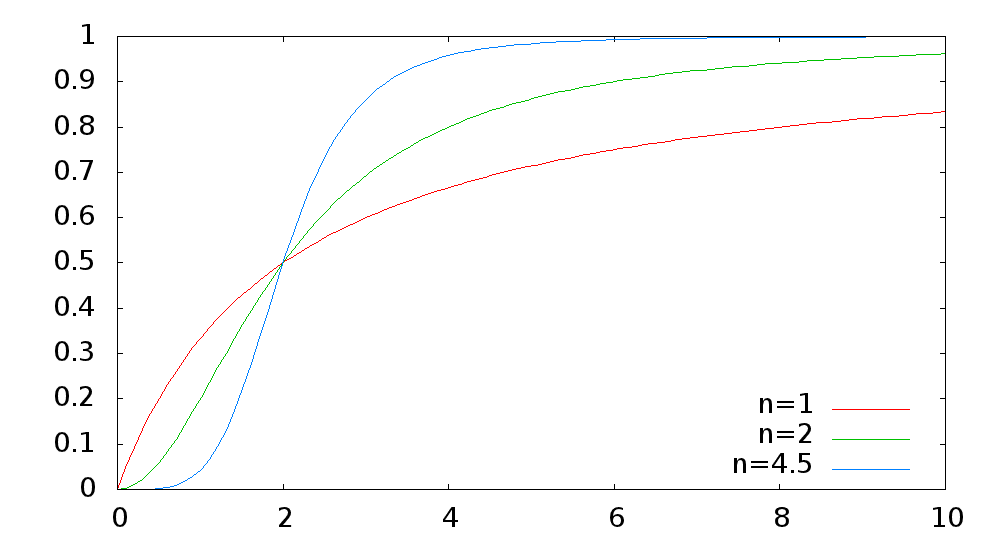
\includegraphics[width=1\textwidth]{hill_factor}
	\caption{Faktor $n$ Hillovej kinetiky pre ve\v lkosti $1, 2$ a $4.5$ ($K_m = 2$)}
	\label{fig:factor}
\end{figure}

%------------------------------------------------------------------------------------------- 
\section{Model checking}
\label{sec:modelChecking}
Model checking alebo overovanie modelov je automatizovan\'a technika form\'alnej verifik\'acie \v specifikovan\'ych vlastnost\'i kone\v cn\'eho stavov\'eho 
syst\'emu. Hlavnou v\'yzvou tejto problematiky je \'uspe\v sne si poradi\v t s probl\'emom expl\'ozie stavov\'eho priestoru (z \textit{ang.} state space
explosion).

Proces overovania modelov pozost\'ava z nasleduj\'ucich pod\'uloh:
\begin{description}
\item[Modelovanie] 
Prvou \'ulohou je prevedenie sk\'uman\'eho syst\'emu do form\'alneho matematick\'eho modelu, ktor\'y bude akceptovan\'y vybran\'ym overovac\'im n\'astrojom.
V niektor\'ych pr\'ipadoch je to \v lahk\'a \'uloha, av\v sak v in\'ych je potreba pou\v zi\v t vhodn\'e abstrakcie za \'u\v celom odstr\'anenia 
irelevantn\'ych detailov alebo naopak zv\'yraznenia ist\'ych \v crtov sk\'uman\'eho syst\'emu.
\item[\v Specifik\'acia]
E\v ste pred samotn\'ym overovan\'im, je nevyhnutn\'e \v specifikova\v t vlastnosti, ktor\'e m\'a sk\'uman\'y syst\'em sp\'l\v na\v t, preto\v ze pr\'ave tie
budeme \v dalej overova\v t. \v Specifik\'aciou sa mysl\'i pou\v zitie nejak\'eho vhodn\'eho formalismu. Typicky napr\'iklad tempor\'alnej logiky, ktor\'a
umo\v z\v nuje sk\'uma\v t spr\'avanie syst\'emu v \v case. My budeme pou\v z\'iva\v t LTL (vi\v d \ref{sec:logika}).
\item[Overovanie]
Model checking dok\'a\v ze overi\v t, \v ci model vyhovuje danej \v specifik\'acii, ale nedok\'a\v ze rozhodn\'u\v t, \v ci dan\'a \v specifik\'acia 
pokr\'yva v\v setky vlastnosti, ktor\'ym sk\'uman\'y syst\'em vyhovuje. Toto je ve\v lmi v\'yznamn\'y probl\'em form\'alneho overovania modelov.

V\'ysledkom overovanie modelu je bu\v d tvrdenie \'ano (v zmysle model sp\'l\v na vlastnos\v t) alebo nie (model nesp\'l\v na vlastnos\v t) a v tomto pr\'ipade
by mal pou\v zit\'y n\'astroj poskytn\'u\v t mo\v znos\v t trasovania chyby (z~\textit{ang.} error trace). T\'ato chybov\'a trasa grafom sa obvykle 
pou\v z\'iva ako protipr\'iklad k overovanej vlastnosti. S jej pomocou m\^ o\v zeme lep\v sie pochopi\v t d\^ ovod a miesto vzniku chyby a upravi\v t syst\'em 
pod\v la toho. \cite{Clarke:MC:Process}
\end{description}

Prv\'e algoritmy pre overovanie modelov pou\v z\'ivali ako formalizmus matematick\'eho modelu dan\'eho syst\'emu Kripkeho \v strukt\'uru. Je to obdoba 
nedeterministick\'eho kone\v cn\'eho automatu (vi\v d kapitolu \ref{sec:buchi}), ktor\'eho stavy s\'u ozna\v cen\'e v\'yrazmi z mno\v ziny $2^{AP}$, kde 
$AP$ s\'u atomick\'e propoz\'icie formule $f$ (vi\v d kapitolu \ref{sec:logika}). V\v setky tieto stavy s\'u akceptuj\'uce.

Nesk\^ or sa pou\v z\'ival $\mu$-kalkulus, ale v s\'u\v casnosti s\'u najroz\v s\'irenej\v s\'im formalizmom automaty. Konkr\'etne budeme pojedn\'ava\v t 
o pou\v zit\'i B\"uchiho automatu (vi\v d kapitolu \ref{sec:buchi}). Tento je ve\v lmi vhodn\'y, preto\v ze sa s jeho pomocou d\'a vyjadri\v t rovnako
model syst\'emu, ako aj po vynalo\v zen\'i ur\v cit\'eho v\'ypo\v ctov\'eho \'usilia, \v specifik\'acia vlastnosti.

Prvou f\'azou tvorby modelu syst\'emu je vytvorenie Kripkeho \v strukt\'ury, ktor\'a sa ale ve\v lmi jednoducho prevedie na automat $\mathcal{A}$. 
\v Specifik\'aciu vlastnosti m\^ o\v zeme vyjadri\v t ako automat $\mathcal{S}$. Potom s\'u oba tieto automaty vytvoren\'e nad rovnakou abecedou 
$\Sigma = 2^{AP}$. Overenie modelu teraz znamen\'a jednoducho zisti\v t, \v ci plat\'i $\mathcal{L(A)} \subseteq \mathcal{L(S)}$, kde $\mathcal{L(A)}$ je 
jazyk zodpovedaj\'uci automatu $\mathcal{A}$ a 
$\mathcal{L(S)}$ je jazyk zodpovedaj\'uci automatu $\mathcal{S}$ (Jazyk je mno\v zina v\v setk\'ych slov, ktor\'e je mo\v zno vygenerova\v t 
pr\'islu\v sn\'ym automatom.). To znamen\'a, \v ze ka\v zd\'e chovanie modelovan\'eho syst\'emu, ur\v cen\'eho jazykom $\mathcal{L(A)}$ sa nach\'adza medzi
povolen\'ymi chovaniami, ur\v cen\'ymi jazykom \v specifik\'acie $\mathcal{L(S)}$.

Toto tvrdenie m\^ o\v zeme preformulova\v t. Nech $\overline{\mathcal{L(S)}}$ je komplement k $\mathcal{L(S)}$, potom pri overovan\'i modelu dokazujeme, \v ci
plat\'i $\mathcal{L(A)} \cap \overline{\mathcal{L(S)}} = \emptyset$. Ak je tento prienik nepr\'azdny, predstavuje to chovanie, ktor\'e je protipr\'ikladom 
k overovanej vlastnosti. Pou\v zi\v t predch\'adzaj\'ucu formul\'aciu n\'am umo\v z\v nuje vedomos\v t, \v ze B\"uchiho automaty s\'u uzavret\'e na prienik
a doplnok (komplement). V\v daka tomu m\^ o\v zeme urobi\v t nasledovn\'e:
\begin{align*}
\emptyset =\ &\mathcal{L(A)} \cap \mathcal{L(S^{'})} = \mathcal{L(A \cap S^{'})} = \mathcal{L(M)},\\
&\textrm{kde } \mathcal{M} = \mathcal{A \cap S^{'}} \textrm{ a }\ \mathcal{S^{'}}= \mathcal{S(\neg\phi)},\\
&\textrm{kde } \mathcal{\phi} \textrm{ je LTL formula a } \mathcal{\neg\phi} \textrm{ jej neg\'acia},
\end{align*}
potom $\mathcal{S^{'}}$ je komplement $\mathcal{S(\phi)}$ a v skuto\v cnosti dokazujeme pr\'azdnos\v t jazyka $\mathcal{L(M)}$ 
(Pre \'uplnos\v t treba doda\v t, \v ze $\mathcal{S(\phi)}$ je automat $\mathcal{S}$ zkon\v struovan\'y zo \v specifik\'acie vlastnosti $\phi$.).

V\'yhodou pou\v zitia automatov pre vyjadrenie modelu sk\'uman\'eho syst\'emu aj  \v specifik\'acie vlastnosti je, \v ze sta\v c\'i skon\v struova\v t automat
pre vlastnos\v t (vi\v d kapitolu \ref{sec:ltltoba}) a automat modelu sa kon\v struuje za behu samotn\'eho overovania pomocou algoritmu pre prienik automatov. 
To znamen\'a, \v ze v mnoh\'ych pr\'ipadoch m\^ o\v zeme vyvr\'ati\v t splnite\v lnos\v t ove\v la sk\^ or, ne\v z sa vytvor\'i cel\'y stavov\'y priestor
automatu modelu n\'ajden\'im prv\'eho protipr\'ikladu. \v Co zna\v cne \v setr\'i \v cas a priestor. T\'ato technika sa naz\'yva overovanie modelu za behu (z \textit{ang.} on"~the"~fly model checking).
\cite{Clarke:MC:BA}

%-------------------------------------------------------------------------------------------
\subsection{Prevod LTL do BA}
\label{sec:ltltoba}
Ako sme u\v z predt\'ym nieko\v lko kr\'at spomenuli, prevod LTL formule na B\"uchiho automat nie je primit\'ivny algoritmus. V skuto\v cnosti je pr\'ili\v s
rozsiahly pre na\v se potreby zoznamovania sa s problematikou. Z tohto d\^ ovodu ho tu nebudeme rozobera\v t, av\v sak uvedieme nieko\v lko d\^ ole\v zit\'ych 
inform\'acii, ktor\'e sa tohto probl\'emu t\'ykaj\'u.

E\v ste pred za\v ciatkom sa mus\'i samotn\'a LTL formula $\phi$ previes\v t do negat\'ivnej norm\'alnej formy (z \textit{ang.} negation normal form). 
Najsk\^ or sa preformuluj\'u niektor\'e tempor\'alne oper\'atory:
\begin{itemize}
\item $\mathbf{F}\ \phi \ \Rightarrow \ \mathbf{true\ U}\ \phi$
\item $\mathbf{G}\ \phi \ \Rightarrow \ \mathbf{false\ R}\ \phi$
\end{itemize}
a tie\v z logick\'e oper\'atory, tak aby zostali iba $\wedge$, $\vee$ a $\neg$. V poslednom kroku pr\'ipravy s\'u v\v setky neg\'acie presunut\'e dovn\'utra:
\begin{itemize}
\item $\neg(\psi\ \mathbf{U}\ \phi) \ \Rightarrow \ (\neg\psi)\ \mathbf{R}\ (\neg\phi)$
\item $\neg(\psi\ \mathbf{R}\ \phi) \ \Rightarrow \ (\neg\psi)\ \mathbf{U}\ (\neg\phi)$
\item $\neg(\mathbf{X}\ \phi) \ \Rightarrow \ \mathbf{X}\ (\neg\phi)$
\end{itemize}

\v Dalej pokra\v cuje dlh\'y algoritmus \cite{Clarke:MC:LTLtoBA}, ktor\'eho v\'ysledkom je B\"uchiho automat $\mathcal{S}$. Jeho kon\v strukcia m\'a exponenci\'alnu \v casov\'u
aj priestorov\'u zlo\v zitos\v t z\'avisl\'u od ve\v lkosti formule $\phi$. Av\v sak v praxi b\'yva takto skon\v struovan\'y automat ovykle men\v s\'i.

Je d\^ ole\v zit\'e e\v ste raz pripomen\'u\v t, \v ze pri overovan\'i modelu vlastne nezis\v tujeme, \v ci model sp\'l\v na vlastnos\v t, ale naopak 
zis\v tujeme, \v ci model nesp\'l\v na opak vlastnosti. D\^ ovodom k tomu je, \v ze je v\'ypo\v ctovo \v lah\v sie vytvori\v t automat z neg\'acie vlastnosti,
ako vytvori\v t komplement automatu z p\^ ovodnej vlastnosti, ktor\'y by mohol ma\v t a\v z dvojn\'asobne exponenci\'alnu priestorov\'u zlo\v zitos\v t.
\cite{Clarke:MC:LTLtoBA}

%-------------------------------------------------------------------------------------------
\subsection{Farebn\' y model checking}
\label{sec:coloredMC}
Farebn\'y model checking alebo tie\v z paraleln\'y sa sna\v z\'i vysporiada\v t s parametriz\'aciou form\'alneho modelu, ktor\'a ho roz\v siruje o nov\'y
rozmer. Ak sa budeme na jednotliv\'e parametre $p_i \in P$, kde $P$ je mno\v zina v\v setk\'ych nezn\'amych parametrov d\'iva\v t ako na intervaly alebo 
sk\^ or ako na mno\v ziny hodn\^ ot, v\v daka diskretiz\'acii. Potom kombin\'acia evaluaci\'i v\v setk\'ych nezn\'amych parametrov tvor\'i parametrick\'y
priestor $\mathcal{P} = \prod_{i = 1}^n [min(p_i),max(p_i)]$, kde $n = |P|$. Tento roz\v siruje model syst\'emu o parametrizovan\'e multi"~afinn\'e funkcie 
$f_i(x,\pi_i)$, kde $\pi_i \in \mathcal{P}$ namiesto be\v zn\'ych multi"~afinn\'ych funkci\'i $f_i(x)$, kde $x = (x_1,\dots{},x_n)$ je vektor premenn\'ych
a $f = (f_i,\dots{},f_n) : \mathbb{R}^n \rightarrow \mathbb{R}^n$ je vektor multi"~afinn\'ych funkci\'i (vi\v d kapitolu \ref{sec:model}). Hodnota $\pi_i$
vyjadruje konkr\'etnu evalu\'aciu parametrov v celom modeli a ozna\v cujeme ju ako farba.

Aby sa zabr\'anilo opakovan\'emu vytv\'araniu automatu pre ka\v zd\'u evalu\'aciu $\pi_i$ za \'u\v celom overenia modelu, bola vytvoren\'a nov\'a pomocn\'a
\v strukt\'ura pomenovan\'a parametrizovan\'a Kripkeho \v strukt\'ura (\v dalej len PKS). T\'a v sebe tradi\v cne uchov\'ava cel\'y stavov\'y priestor modelu,
ale navy\v se s novou inform\'aciou, ktor\'a rozhoduje pod ktorou farbou, resp. konkr\'etnou evalu\'aciou parametrov sa d\'a prejs\v t z prechodu $s$ 
do prechodu $s^{'}$. Ka\v zd\'y prechod mus\'i by\v t uschopnen\'y aspon pod jednou farbou, ale z\'arove\v n m\^ o\v ze by\v t aj pod v\v setk\'ymi. Cel\'y
stavov\'y priestor je tak zjednotenie v\v setk\'ych jednofarebn\'ych stavov\'ych priestorov.

V\v daka tomu prebieha overovanie v\v setk\'ych parametriz\'aci\'i modelu naraz. V\'ysledkom je najv\"a\v c\v sia mno\v zina parametriz\'aci\'i, v ktor\'ych
model sp\'l\v na dan\'u vlastnos\v t. \cite{TCBB-2010}

%====================================MODEL==================================================
\chapter{Biochemick\'y dynamick\'y vstupn\'y model}
\label{sec:model}
T\'ato kapitola je z ve\v lkej miery doslovne citovan\'a z ni\v z\v sie uveden\'ych zdrojov.
\\

\noindent
\it A. \ Multi-afinn\'y ODE model\rm
\\

Vstupn\'ym modelom sa u n\'as mysl\'i model biochemick\'ych reakci\'i, ktor\'y je v na\v som po\v nat\'i bran\'y ako po \v castiach 
multi"~afinn\'y syst\'em diferenci\'alnych rovn\'ic. Ale za\v cnime od po\v ciatku a postupne sa dopracujme k tomuto v\'ysledku.

Na z\'aklade pravidla o mass~action kinetike (vi\v d \ref{sec:massAction}) je mo\v zn\'e modelova\v t \v lubovoln\'u biochemick\'u reakciu alebo dokonca 
s\'ustavu tak\'ychto reakci\'i pomocou s\'ustavy neline\'arnych ODE \cite{ODE}.

Uva\v zujme multi"~afinn\'y syst\'em vo forme $\dot{x} = f(x)$, kde $x = (x_1,\dots{},x_n)$ je vektor premenn\'ych a $f = (f_1,\dots{},f_n)$ \ : \ 
$\mathbb{R}^n \rightarrow \mathbb{R}^n$ je vektor multi"~afin\-n\'ych funkci\'i. Tieto funkcie s\'u vlastne polyn\'omy, v ktor\'ych je stupe\v n premenn\'ych 
$x_1,\dots{},x_n$ obmedzen\'y na hodnotu 1. Ka\v zd\'a premenn\'a $x_i$, kde $i \in \{1,\dots{},n\}$ predstavuje koncentr\'aciu \v specifickej chemickej l\'atky a je interpretovan\'a ako
{$\mathbb{R}_+ = \lbrace{}  x \in \mathbb{R}\ |\ {}x \geq 0  \rbrace$}. /*Mozno priklad*/

Z d\^ ovodu, \v ze premenn\'e m\^ ozeme vyjadri\v t len ako nez\'aporn\'e re\'alne \v cisla, je mo\v zn\'e tie\v z spojit\'y stavov\'y priestor na\v seho 
matematick\'eho syst\'emu obmedzi\v t iba na prv\'y, resp. kladn\'y kvadrant {$\mathbb{R}_+^n = \lbrace{}  x \in \mathbb{R}^n\ |\ {}x \geq 0  \rbrace$}.

Ak uva\v zujeme o premenn\'ych ako o nestabiln\'ych chemick\'ych l\'atkach, ktor\'e sami od seba degraduj\'u v \v case, m\^ o\v zme s k\v ludom obmedzi\v t 
n\'a\v s spojit\'y stavov\'y priestor $\mathcal{D}$ e\v ste viac. A s\'ice na $n$"~dimenzion\'alny obd\'l\v znik $\mathcal{D} = \prod_{i=1}^n[0,max_i] 
\subset \mathbb{R}^n$, kde $max_i$ je horn\'a hranica koncentr\'acie pre\-men\-nej $x_i$.
\cite{HIBI-2009}\cite{HIBI-2010}
\\

\noindent
\it B. \ Po \v castiach multi"~afinn\'y ODE model\rm
\\

Multi"~afinn\'y syst\'em diferenci\'alnych rovn\'ic dok\'a\v ze pokry\v t skoro cel\'u mass~action kinetiku s jedinou v\'ynimkou. A tou s\'u 
homodim\'ery a reakcie s nimi spojen\'e. D\^ ovodom je predch\'adzaj\'uce obmedzenie multi"~afinn\'ych funkci\'i $f_1,\dots{},f_n$ s oh\v ladom 
na stupe\v n premenn\'ych $x_1,\dots{},x_n$.

Teoreticky sme schopn\'y  pop\'isa\v t ak\' yko\v lvek biochemick\'y model pomocou pravidiel tejto kinetiky. V skuto\v cnosti, ak sa pok\'usime formulova\v t 
tieto pravidl\'a pre rozsiahly model, zist\'ime, \v ze s narastaj\'ucou ve\v lkos\v tou rastie komplexita t\'ychto pravidiel a navy\v se k \'uplnosti modelu
je potrebn\'e pozna\v t ve\v lk\'e mno\v zstvo \v co najpresnej\v sie vy\v c\'islen\'ych parametrov. Pr\'ave tento druh\'y probl\'em m\^ o\v ze by\v t 
v niektor\'ych pr\'ipadoch experiment\'alne nerie\v site\v ln\'y. \v Ci u\v z ide o ve\v lk\'e enzymatick\'e komplexy, alebo (o l\'atky s ve\v lmi 
kr\'atkou existenciou / o ve\v lmi r\'ychlo degraduj\'ujce l\'atky).

Pr\'ave preto sa pon\'ukaj\'u mo\v znosti aproxim\'acie, ktor\'e nie len zmen\v suj\'u syst\'em a t\'ym aj dimenzionalitu matematick\'eho modelu, 
ale zjednodu\v suj\'u aj v\'ypo\v ctov\'u zlo\v zitos\v t. Takouto mo\v znos\v tou je aj aproxim\'acia kv\'azistacion\'arneho stavu (vi\v d \ref{kinetiky}.B). 
Napr\'iklad Michaelis"~Mentenovej kinetika (vi\v d. \ref{kinetiky}), 
\v ci obecnej\v sia Hillova kinetika (vi\v d. \ref{kinetiky}.C) a tie\v z sigmoid\'alne prep\'ina\v ce publikovan\'e na konferencii CAV (Grosu et al. 2011)
\cite{CAV-2011}. 
V\v setky vy\v s\v sie zmienen\'e abstrakcie n\'a\v s n\'astroj pon\'uka a budeme ich jednotne ozna\v cova\v t ako regula\v cn\'e funkcie $\rho(x)$, ktor\'e
budeme matematicky definova\v t nesk\^ or. 

Takto redukovan\' e difernci\'alne rovnice maj\'u formu 
racion\'alnych polyn\'omov, z\'iskan\'ych ako line\'arna kombin\'acia t\'ychto regula\v cn\'ych funkc\'i, 
medzi ktor\'e patria aj Heavisideove alebo schodov\'e funkcie \cite{step}. 
V skuto\v cnosti v\'ysledn\'y 
matematick\'y model nie je multi"~afinn\'y, ale na druh\'u stranu je ho mo\v zn\'e aproximova\v t v zmysle po \v castiach mul\-ti"~afin\-n\'eho syst\'emu. 
A to tak, \v ze nahrad\'ime v\v setky regula\v cn\'e funkcie s\'ustavou vhodn\'ych po \v castiach line\'arnych rampov\'ych funkci\'i. Tieto s\'u definovan\'e 
nasledovne:
\begin{align*}
	r^+coor (x_i,\theta{}_i,\theta{}_i^{'},y,y^{'}) \ = \left\{ \begin{array}{cl}
y, & \textrm{pre} \ x_i < \theta_i,\\
y + (y^{'} - y)\frac{x_i - \theta_i}{\theta_i^{'} - \theta_i}, & \textrm{pre} \ \theta_i < x_i < \theta_i^{'},\\
y^{'}, & \textrm{pre} \ x_i > \theta_i^{'}.
	\end{array}
	\right.;
	\\
	\\
	\centerline{$r^+ (x_i, \theta{}_i, \theta{}_i^{'}, a,b) \ = \ r^+coor (x_i,\theta{}_i,\theta{}_i^{'},a\theta_i + b,a\*\theta_i^{'} + b)$;}
\end{align*}
\begin{align*}
	\textrm{kde} \ &i \in \{1,\dots{},n\},\\
	&y = x_j, y^{'} = x_j^{'}; j \in \{1,\dots{},n\} \wedge j \neq i,\\
	&\theta_i, \theta_i^{'} \in \mathbb{R}^+, \ \theta_i < \theta_i^{'} \leq max_i,\\
	&a, b \in \mathbb{R}.
\end{align*}

Potom klesaj\'uce rampov\'e funkcie s\'u definovan\'e ako kvantitat\'ivny doplnok rast\'ucich:
\begin{align*}
r^-coor (x_i,\theta{}_i,\theta{}_i^{'},y,y^{'}) &\ = \ 1 - r^+coor (x_i,\theta{}_i,\theta{}_i^{'},y,y^{'})\\
r^- (x_i, \theta{}_i, \theta{}_i^{'}, a,b) &\ = \ 1 - r^+ (x_i, \theta{}_i, \theta{}_i^{'}, a,b)
\end{align*}

U\v z zmienen\'e regula\v cn\'e funkcie maj\'u nasleduj\'uce formy:
\begin{align*}
hill^+(x_i, \theta_i, d, a, b) &\ = \ a + (b - a)\frac{[x_i]^d}{[\theta_i]^d + [x_i]^d};\\
hill^+(x_i, \theta_i, d, a, b) &\ = \ 1 - hill^+(x_i, \theta_i, d, a, b);\\
\\
s^+(x_i, e, \theta_i, a, b) &\ = \ a + (b - a)\frac{1 + tanh(e(x_i - \theta_i))}{2};\\
s^-(x_i, e, \theta_i, a, b) &\  = \ 1 - s^+(x_i, e, \theta_i, a, b);\\
\\
h^+(x_i,\theta_i,a,b) &\ = \ a,\ \textrm{ak}\ x_i < \theta_i;\ b\ \textrm{inak};\\
h^-(x_i,\theta_i,a,b) &\ = \ 1 - h^+(x_i,\theta_i,a,b);
\end{align*}
\begin{align*}
\textrm{kde}\ &hill^+, hill^- \textrm{s\'u funkcie Hillovej kinetiky,}\\
&s^+, s^- \textrm{s\'u sigmoid\'alne prep\'ina\v ce},\\
&h^+, h^- \textrm{s\'u Heavisideove (schodov\'e) funkcie},\\
&\theta_i \in \mathbb{R}^+, \ \theta_i \leq max_i,\\
&i \in \{1,\dots{},n\},\\
&a, b \in \mathbb{R}_0^+,\\
&e, d \in \mathbb{R}^+.
\end{align*}

\noindent\v Speci\'alnym pr\'ipadom je recipro\v cn\'a hodnota sigmoid\'alnej funkcie:
\begin{align*}
s^+(x_i, e, \theta_i, a, b)^{-1} \ = \ s^-(x_i, e, \theta_i + \frac{ln(\frac{a}{b})}{2e}, b^{-1}, a^{-1}),
\end{align*}
ktor\'u ozna\v cujeme ako $s^+inv(x_i, e, \theta_i, a, b)$. Potom klesaj\'ucu recipro\v cn\'u funkciu ozna\v c\'ime obdobne ako doplnok rast\'ucej:
\begin{align*}
\centerline{$s^-inv(x_i, e, \theta_i, a, b) \ = \ 1 - s^+(x_i, e, \theta_i, a, b)$.}
\end{align*}D\^ okaz mo\v zno n\'ajs\v t v \v cl\'anku \textit{From cardiac cells to genetic regulatory network} na strane 6 \cite{CAV-2011}.

Teraz u\v z m\^ o\v zeme zadefinova\v t \'upln\'y form\'at n\'a\v sho po \v castiach multi"~a\-fin\-n\'eho ODE modelu 
(\v dalej len PMA model z \textit{ang.} piece"~wise multi"~affine ODE model). PMA model $\mathcal{M}$ je dan\'y ako $\dot{x} = f(x)$, 
kde $x$ je st\'ale vektor premenn\'ych $(x_1,\dots{},x_n)$, ale $f = (f_1,\dots{},f_n)$ : $\mathbb{R}^n \rightarrow \mathbb{R}^n$ je tentokr\'at vektor 
po \v castiach multi"~afinn\'ych funkci\'i. Nevyhnutnou s\'u\v cas\v tou modelu $\mathcal{M}$ je mno\v zina prahov\'ych hodn\^ ot (z \textit{ang.} threshold)
$\theta_m^i \in \mathbb{R}^+$ sp\'l\v naj\'uca $min_i = \theta_1^i < \theta_2^i < \dots{} < \theta_{\eta_i}^i = max_i$, kde $i \in \{1,\dots{},n\}$, 
$m \in \{1,\dots{},\eta_i\}$ a plat\'i, \v ze $\eta_i \geq 2$.

Uva\v zujme $\Omega$ ako \v cas\v t modelu $\mathcal{M}$ tak, \v ze $\Omega = \prod_{i = 1}^n\{1,\dots{},\eta_i - 1\}$. Funkcia 
$g : \mathbb{R}^n \rightarrow \mathbb{R}^+$ je vtedy po \v castiach multi"~afinn\'a, ak je multi"~afinn\'a na ka\v zdom $n$-dimenzion\'alnom intervale
$(\theta_{j_1}^1,\theta_{j_1 + 1}^1)\times \dots{} \times (\theta_{j_n}^n,\theta_{j_n + 1}^n)$, kde $(j_1,\dots{},j_n) \in \Omega$ a z\'arove\v n 
$\forall{}i, 1 \leq i \leq n, j_i < max_i$. Potom dost\'avame $n$-dimenzion\'alny PMA model pozost\'avaj\'uci z funkci\'i $f$ v nasleduj\'ucom tvare:
\begin{align}
\label{eq:equationDescribtion}
f_i(x) = \sum (s\underset{j \in I}\prod{\rho_i^j(x)}),
\end{align}
kde $i \in \{1,\dots{},n\}$, $s \in \{-1,1\}$, $I$ je nepr\'azdna podmno\v zina kone\v cnej mno\v ziny indexov v\v setk\'ych pou\v zit\'ych regula\v cn\'ych
funkci\'i a $\rho_i^j$ je pr\'islu\v sn\'a regula\v cn\'a funkcia, ktor\'a m\^ o\v ze nadob\'uda\v t tieto hodnoty:
\begin{align}
\label{eq:regulatingFunctions}
\rho(x_t) = 
\left\{ \begin{array}{cl}
c, &c \in \mathbb{R}\\
%p, &p \in \langle g,h \rangle; \ g,h \in \mathbb{R}\\
x_k, & k \in \{1,\dots{},n\}\\
r^*(x_k,\theta_m^k,\theta_{m+1}^k,a^{'},b^{'}), &m \in \{1,\dots{},\eta_k-1\}; a^{'},b^{'} \in \mathbb{R}\\
r^*coor(x_k,\theta_m^k,\theta_{m+1}^k,x_t,x_t^{'}), &t \in \{1,\dots{},n\} \wedge t \neq i\\
s^*(x_k,e,\theta_m^k,a,b), &e \in \mathbb{R}^+; \ a,b \in \mathbb{R}_0^+\\
s^*inv(x_k,e,\theta_m^k,a,b),\\
hill^*(x_k,\theta_m^k,d,a,b), &d \in \mathbb{R}^+\\
h^*(x_k,theta_m^k,a,b)
\end{array} \right. ,
\end{align}
kde $* \in \{+,-\}$. Ak $\rho_i^{j_1}, \rho_i^{j_2}$ s\'u regula\v cn\'e funkcie, ktor\'e patria do jednoho produktu $s\underset{j \in I}\prod\rho_i^j(x)$,
tak \v ze $j_1, j_2 \in I$, mus\'i plati\v t $dep(\rho_i^{j_1})\ \cap\ dep(\rho_i^{j_2}) = \emptyset$, kde $dep(\rho)$ je mno\v zina premenn\'ych $x$,
na ktor\'ych je $\rho$ z\'avysl\'a.
Pr\'iklad PMA modelu mo\v zno n\'ajs\v t na obr\'azku ... 

Do modelu je priamo zaveden\'a aj mo\v znos\v t zadania kon\v stantnej funkcie (v pr\'ipade, \v ze $\rho(x_t) = c$) a line\'arnej funkcie 
(v pr\'ipade $\rho(x_t) = x_k$). \v Dal\v sou nevyhnutnou s\'u\v cas\v tou modelu s\'u inici\'alne podmienky, vyjadruj\'uce 
po\v ciato\v cn\'e koncentr\'acie jednotliv\'ych l\'atok. Tieto nie s\'u vyjadren\'e presne, ale namiesto toho s\'u ur\v cen\'e intervalom, ktor\'eho
hranice musia by\v t z mno\v ziny $\{ \theta_1^i,\dots{},\theta_{\eta_i}^i \}$.

Takto vytvoren\'y model je prakticky pou\v zite\v ln\'y pre \v lubovoln\'y biologick\'y syst\'em.
\cite{HIBI-2009}\cite{HIBI-2010}

%-------------------------------------------------------------------------------------------
\section{Abstrakcia}
\label{sec:abstraction}

\noindent
\textit{A. \ Optim\'alna line\'arna abstrakcia}
\\

V minulej \v casti sme objasnili, pre\v co je potrebn\'e prev\'adza\v t regula\v cn\'e funkcie $\rho(x_i)$, kde $x_i$ je premenn\'a na po \v castiach line\'arne 
rampov\'e funkcie. V tejto \v casti sa pok\'usime objasni\v t princ\'ip tohto prevodu. Vyn\'ara sa hne\v d nieko\v lko probl\'emov:
\begin{enumerate}
\item Ako vhodne rozdeli\v t \v lubovoln\'u krivku na zadan\'y po\v cet r\'amp.
\item Ako vhodne rozdeli\v t nieko\v lko kriviek rovnakej dimenzie na zadan\'y po\v cet r\'amp.
\item Ako vybra\v t spr\'avny po\v cet r\'amp, tak aby stavov\'y syst\'em nebol pr\'ili\v s ve\v lk\'y a z\'arove\v n tak, aby abstrakcia nebola 
pr\'ili\v s hrub\'a.
\end{enumerate}
Na prv\'u ot\'azku d\'ava odpove\v d algoritmus dynamick\'eho programovania vyvinut\'y pre po\v c\'ita\v cov\'u grafiku, konkr\'etne pre aproxim\'aciu
digitalizovan\'ych polygon\'alnych kriviek s minim\'alnou chybou \cite{CURVES}. Tento bol upraven\'y a roz\v s\'iren\'y pre viacero kriviek naraz v 
\v cl\'anku \textit{From Cardiac Cells to Genetic Regulatory Network} (Grosu et al.) \cite{CAV-2011} a to tak, \v ze zmienen\'a chyba sa po\v c\'ita pre
v\v setky krivky naraz. Aby to bolo mo\v zn\'e, musia by\v t v\v setky krivky diskretizovan\'e v rovnak\'ych $x$-ov\'ych bodoch. 
V na\v som pr\'ipade sa krivkami myslia Hillove funkcie (vi\v d \ref{kinetiky}.C) a sigmoid\'alne funckie pop\'isan\'e, tie\v z v \v cl\'anku \cite{CAV-2011}.

\' U\v celom tejto abstrakcie je n\'ajs\v t tak\'e body $x_i$, kde $i \in \{1,\dots{},n\}$ a $n$ je po\v cet diskretiza\v cn\'ych bodov, ktor\'e bud\'u 
seka\v t krivky na line\'arne segmenty s minim\'alnou odch\'ylkou (chybou). Chyba sa po\v c\'ita ako s\'u\v cet druh\'ych mocn\'in vzdialenost\'i dvoch bodov 
na $y$-ovej ose. T\'ymito bodmi s\'u funk\v cn\'a hodnota krivky a funk\v cn\'a honota rampy pre konkr\'etny bod $x_i$ na \'useku ohrani\v cenom bodmi 
$x_a$ a $x_b$, kde $x_i \in \langle x_a,x_b\rangle$. Rampa je v tomto zmysle bran\'a ako line\'arna spojnica medzi funk\v cn\'ymi hodnotami t\'ychto
hrani\v cn\'ych bodov. Ak sa n\'ajde vyhovuj\'uca hodnota chyby, potom mo\v zno s istotou tvrdi\v t, \v ze body $x_a$ a $x_b$ s\' u z\'arove\v n 
hrani\v cn\'ymi bodmi nov\'eho segmentu. So v\v setk\'ymi takto z\'iskan\'ymi bodmi u\v z nie je probl\'em previes\v t ka\v zd\'u funkciu na jej po \v castiach 
line\'arnu formu. Z\'arove\v n treba tieto body ulo\v zi\v t ako nov\'e prahov\'e hodnoty modelu (vi\v d kapitolu \ref{sec:model}.B). 
Pr\'iklad abstrakcie mo\v zno vidie\v t na obr\'azku \ref{fig:noabstract}.
\begin{figure}[t]
	\label{fig:noabstract}
    \centering
    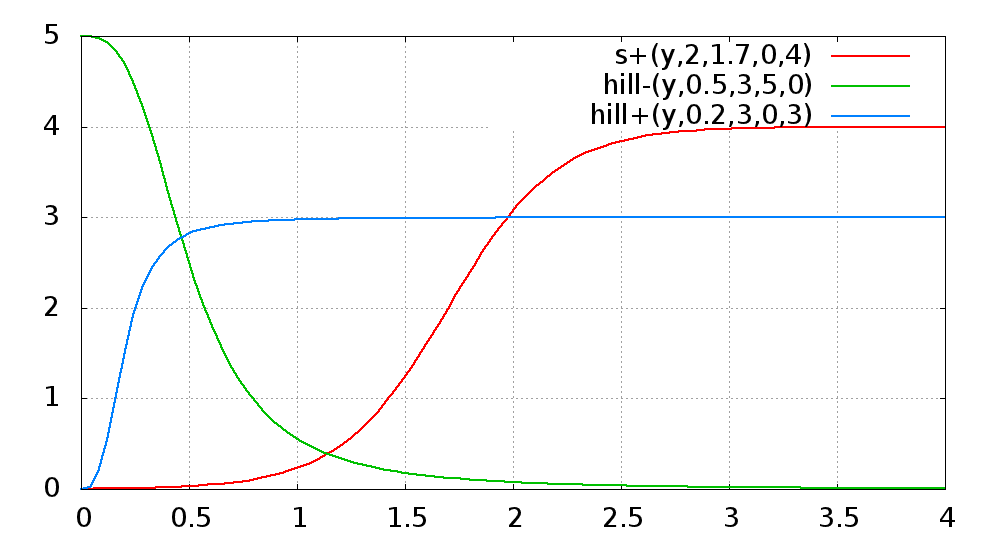
\includegraphics[width=1\textwidth]{abstractNO}
    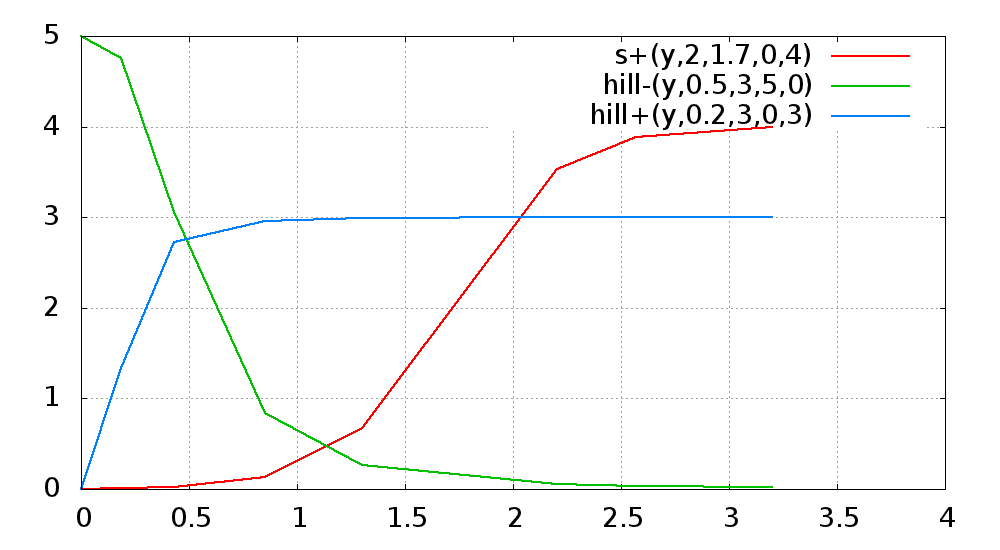
\includegraphics[width=1\textwidth]{abstractYES}
    \caption{Tri krivky s popisom. V prvom pr\'ipade bez pou\v zitia abstrakcie a v druhom preveden\'e na s\'ustavu r\'amp po pou\v zit\'i abstrakcie 
    s parametrami: diskretiza\v cn\'ych bodov $500$, po\v zadovan\'y po\v cet segmentov $7$.}
\end{figure}

Odpove\v d na tretiu ot\'azku oh\v ladom spr\'avneho po\v ctu r\'amp je tak\'ato.
U\v z\'ivate\v l mus\'i nastavi\v t po\v zadovan\'y po\v cet s\'am, to mu v\v sak umo\v z\v nuje, aby sk\'u\v sal r\^ ozne \'urovne abstrakcie osobne.
\cite{CAV-2011}
\\

\noindent
\textit{B. \ Obd\'l\v znikov\'a abstrakcia}
\\

V\'yhodou multi"~afinn\'eho syst\'emu je, \v ze ho mo\v zno abstrahova\v t do podoby obd\'l\v znikov\'eho prechodov\'eho syst\'emu (z \textit{ang.}
Rectangular Abstraction Transition System, skr\'atene RATS) \cite{RATS}. K tomu je potreba p\^ ovodn\'y $n$-dimenzion\'alny syst\'em, kde $n$ je po\v cet 
premenn\'ych najsk\^ or rozdeli\v t na men\v sie $n$-dimenzion\'alne oddiely. Ka\v zd\'a premenn\'a m\'a priraden\'u mno\v zinu prahov\'ych hodn\^ ot alebo
thresholdov, ktor\'e vyjadruj\'u v\'yznamn\'e, \v ci zauj\'imav\'e koncentra\v cn\'e hladiny. Ka\v zdej premennej s\'u priraden\'e aspo\v n dve tak\'eto 
hodnoty a to minim\'alna a maxim\'alna. \v Dal\v sie m\^ o\v zu by\v t zadefinovan\'e vo vstupnom modeli, alebo m\^ o\v zu poch\'adza\v t z predch\'adzaj\'ucej
line\'arnej abstrakcie.

Teraz u\v z nie je probl\'em rozdeli\v t multi"~afinn\'y syst\'em pod\v la t\'ychto prahov na men\v sie $n$-rozmern\'e ohrani\v cen\'e \v casti nazvan\'e 
obd\'l\v zniky. Tieto si m\^ o\v zeme predstavi\v t ako uzly grafu. Ak s\'u dva obd\'l\v zniky susedmi, m\^ o\v ze medzi nimi vznikn\'u\v t prechod v zmysle
hrany medzi dvoma uzlami. Takto dost\'avame diskr\'etny prechodov\'y syst\'em (RATS) z p\^ ovodne dynamick\'eho syst\'emu. 

Prechody s\'u samozrejme orientovan\'e. Hodnotu orient\'acie dostaneme zo smerov\'ych vektorov vypo\v c\'itan\'ych vo v\v setk\'ych rohoch $n$-rozmern\'eho 
obd\'l\v znika. A to tak, \v ze ak aspo\v n jeden vektor v rohoch spolo\v cn\'ych so susediacim obd\'l\v znikom m\'a smer k tomuto susedovi, prid\'ame 
odch\'adzaj\'ucu hranu z tohto tohto uzla do susedn\'eho. Ak aspo\v n jeden vektor v rohoch spolo\v cn\'ych so susediacim obd\'l\v znikom m\'a smer od tohto
suseda, prid\'ame prich\'adzaj\'ucu hranu zo susediaceho uzla k tomuto uzlu. To znamen\'a, \v ze hrany m\^ o\v zu by\v t aj obojsmern\'e. Podmienkou je, \v ze
ak nastane situ\'acia, kedy uzol nebude ma\v t \v ziadnu odch\'adzaj\'ucu hranu, mus\'ime mu prida\v t slu\v cku. Tento jav symbolizuje rovnov\'a\v zny stav
v dan\'ych podmienkach.

Je zn\'amy fakt, \v ze obd\'l\v znikov\'a absrakcia je nadaproxim\'aciou vzh\v ladom k trajekt\'oriam p\^ ovodn\'eho dynamick\'eho modelu.
\cite{BIODIVINE}

mozno dorobit obrazok podobne ako v \cite{BIODIVINE} pomocou latex/picture


%====================================NASTROJE===============================================
\chapter{V\'ychodiskov\'y stav a podobn\' e n\'astroje}

%-------------------------------------------------------------------------------------------
\section{BioDiVinE 1.0}
\label{sec:biodivine}
P\^ ovodn\'y n\'astroj BioDiVinE bol vyvinut\'y v laborat\'oriu syst\'emovej biol\'ogie (SyBiLa)\cite{sybila} v spolupr\'aci s laborat\'oriom paraleln\'ych 
a distribuovan\'ych syst\'emov (ParaDiSe)\cite{paradise}. Obe s\'idlom na fakulte informatiky Masarykovej univerzity. 

BioDiVinE 1.0 je n\'astroj vytvoren\'y pre verifik\'aciu vlastnost\'i biochemick\'ych modelov zadan\'ych ako syst\'em ODE (vi\v d kapitolu \ref{sec:model}).
Je to nadstavba n\'astroja DiVinE \cite{divine}, ur\v cen\'eho na model checking (vi\v d kapitolu \ref{sec:modelChecking}). K tomuto 
\'u\v celu pon\'uka nieko\v lko odli\v sn\'ych algoritmov.

Vstupom je, ako u\v z bolo povedan\'e biochemick\'y model v tzv. .bio form\'ate (podrobnosti v \cite{sybila-biodivine}), ktor\'y 
m\^ o\v ze predstavova\v t genov\'u regula\v cn\'u sie\v t alebo vz\'ajomn\'u interakciu prote\'inov, \v ci in\'e. D\^ ole\v zitou s\'u\v cas\v tou je aj
s\'ubor s jednou alebo viacer\'ymi vlastnos\v tami zap\'isan\'ymi ako LTL formule (vi\v d kapitolu \ref{sec:logika}). Tieto dva s\'ubory sa musia skombinova\v t
do jednoho pou\v zit\'im pr\'islu\v sn\'eho n\'astroja, pri\v com vlastnos\v t sa z\'arove\v n prevedie z LTL formule na B\" uchiho automat (vi\v d kapitolu 
\ref{sec:buchi}). Takto hotov\'y vstup sa m\^ o\v ze preda\v t jednomu z overovac\'ich algoritmov.

Je vidno, \v ze postup nie je ve\v lmi u\v z\'iva\v te\v lsky pr\'ivetiv\'y. U\v z\'ivate\v l mus\'i najsk\^ or pou\v zi\v t jeden n\'astroj 
pre vytvorenie vstupn\'eho s\'uboru, potom ho ru\v cne premenova\v t, aby ho \v dal\v s\'i n\'astroj, tentokr\'at overovac\'i spr\'avne rozpoznal. V\'ysledky
v podobe protipr\'ikladu alebo podrobn\'y v\'ypis priebehu procesu s\'u vygenerovan\'e do nov\'ych s\'uborov .trail alebo .report po zadan\'i pr\'islu\v sn\'eho
vstupn\'eho prep\'ina\v ca vybran\'eho algoritmu. Jedinou v\'yhodou je, \v ze v\"a\v c\v sina prep\'ina\v cov je unifikovan\'a, preto\v ze n\'astroje boli vytvoren\'e
jedn\'ym v\'yvoj\'arskym t\'imom.

Cel\'y n\'astroj BioDiVinE pritom obsahuje zbyto\v cne ve\v la \v dal\v s\'ich roz\v s\'iren\'i pre in\'e typy modelov, preto\v ze p\^ ovodn\'y n\'astroj 
DiVinE bol prevzat\'y ako celok aj s t\'ymito predch\'adzaj\'ucimi roz\v s\'ireniami.

Kv\^ oli vy\v s\v sie spomenut\'ym d\^ ovodom sme si dali za cie\v l okrem roz\v s\'irenia vstupn\'eho modelu a abstrakcie aj refaktoriz\'aciu star\'eho n\'astroja.
\cite{BIODIVINE}

%-------------------------------------------------------------------------------------------
\section{PEPMC}
N\'astroj vyvinut\'y v laborat\'oriu syst\'emovej biol\'ogie (SYBILA)\cite{sybila} pre overovanie modelov s oh\v ladom na odhad parametrov (z \textit{ang.}
Parameter Estimation by Parallel Model Checking, skr\'atene PEPMC). Funguje na princ\'ipe paraleln\'eho overovania modelov alebo tie\v z farebn\'eho 
overovania modelov (vi\v d kapitolu \ref{sec:coloredMC}). Modelom je syst\'em ODE podobne ako v n\'astroji BioDiVinE 1.0, ale roz\v s\'iren\'y o mo\v znos\v t
zad\'avania po \v castiach line\'arnych ramp funkci\'i (vi\v d kapitolu \ref{sec:model}). D\^ ole\v zit\'ym rozdielom oproti BioDiVinE-u a s\'u\v casne hlavnou
podstatou n\'astroja PEPMC v\v sak je parametriz\'acia modelu a s t\'ym s\'uvisiace preh\v lad\'avanie parametrick\'eho priestoru.

Existuje my\v slienka zl\'u\v ci\v t tieto dva n\'astroje, br\'ani tomu v\v sak mierne odli\v sn\'y vstup, datov\'y model a samozrejme rozdielne jadr\'a 
programov. Nebudeme tu v\v sak tento probl\'em \v dalej rozobera\v t, preto\v ze nie je s\'u\v cas\v tou na\v sej t\'emy.
\cite{HIBI-2010}

%-------------------------------------------------------------------------------------------
\section{RoVerGeNe}
RoVerGeNe je podobne ako PEPMC n\'astroj pre anal\'yzu genetick\'ych regula\v cn\'ych siet\'i s neur\v cit\'ymi parametrami. Model siete je zap\'isan\'y ako
po \v castiach multi"~afinn\'y syst\'em diferenci\'alnych rovn\'ic. Vlastnosti, proti ktor\'ym sa model overuje, maj\'u formu LTL formule a prametre s\'u 
zadan\'e ako intervaly. N\'astroj sa sna\v z\'i overi\v t, \v ci model sp\'l\v na dan\'u vlastnos\v t pre v\v setky parametre.

Na rozdiel od PEPMC v\v sak RoVerGeNe dok\'a\v ze pracova\v t aj s line\'arnymi kombin\'aciami parametrov. To v praxi znamen\'a, \v ze obd\'l\v znikov\'a
abstrakcia (vi\v d \ref{sec:abstraction}.B) u neho nie je
pou\v zite\v ln\'a, preto\v ze vy\v zaduje, aby $n$-dimen\-zion\'alne \v stvoruholn\'iky s ktor\'ymi pracuje, boli ortogon\'alne, \v ci\v ze obd\'l\v zniky.
Namiesto toho pou\v z\'iva tento n\'astroj \v standardn\'e polyhedr\'alne oper\'acie bal\'ika MPT \cite{mpt} a cel\'y je naprogramovan\'y v Matlabe.
\cite{rovergene}
\cite{rovergene-site}

%-------------------------------------------------------------------------------------------
\chapter{BioDiVinE 1.1}
V kapitole \ref{sec:biodivine} boli predstaven\'e niektor\'e nedostatky p\^ ovodn\'eho n\'astroja BioDiVinE 1.0, ktor\'e sme si dali za cie\v l odstr\'ani\v t.
S\'u\v casne bol z\'aujem o~roz\v s\'irenie jeho funkcionality a odstr\'anenie nadbyto\v cn\'ych \v cast\'i k\'odu. 

Prvotn\'y impulz spo\v c\'ival v zov\v seobecnen\'i vstupn\'eho modelu, aby poskytoval \v sir\v s\'i z\'aber mo\v znost\'i. Aby nebol obmedzen\'y iba na mass 
action kinetiku (vi\v d \ref{sec:massAction}) a s t\'ym s\'uvisiace neline\'arne diferenci\'alne rovnice. Do \'uvahy prich\'adzali samozrejme najbe\v znej\v sie 
pou\v z\'ivan\'e Michaelis"~Mente\-novej kinetika a Hillova kinetika (vi\v d \ref{kinetiky}), ale aj Heavisidove funkcie \cite{step}, sigmoid\'alne funkcie z
konferencie CAV 2011 \cite{CAV-2011} a obecn\'e rampov\'e funkcie (vi\v d \ref{sec:model}.B), ktor\'e sl\'u\v zia aj ako produkt optim\'alnej line\'arnej abstrakcie (vi\v d 
\ref{sec:abstraction}.A).

T\'ym sme nak\'usli \v dal\v siu nov\'u funkcionalitu. Zl\'u\v cenie nov\'eho roz\v s\'iren\'eho vstupn\'eho modelu (vi\v d \ref{sec:model}) a p\^ ovodne 
pou\v z\'ivanej obd\'l\v znikovej abstrakcie (vi\v d \ref{sec:abstraction}.B). Prechodom medzi t\'ym je pr\'ave vy\v s\v sie spomenut\'a op\-ti\-m\'al\-na 
line\'arna abstrakcia, ktor\'a prevedie novozaveden\'e nemulti"~afin\-n\'e funk\-cie na po \v castiach multi"~afinn\'e, presne ako je potrebn\'e pre 
obd\'l\v znikov\'u abstrakciu.

Pri z\'apise jednotliv\'ych rovn\'ic modelu sme sa chceli vyhn\'u\v t oper\'acii delenia, preto sme sa rozhodli v\v setky prid\'avan\'e funkcie zapisova\v t
v podstate unifikovan\'ym sp\^ osobom, ktor\'y jasne ur\v cuje o ak\'y typ funkcie sa jedn\'a, \v ci je rast\'uca alebo klesaj\'uca a \v dalej parametre 
nevyhnutn\'e pre jej vy\v c\'islenie. Tak isto sme pridali p\'ar noviniek ako definovanie pomenovan\'ych kon\v st\'ant a volite\v ln\'e, u\v z\'ivate\v lom 
zad\'avan\'e parametre pre line\'arnu abstrakciu. Konkr\'etne ide o po\v cet bodov, v ktor\'ych maj\'u by\v t funkcie evaluovan\'e a o po\v cet segmentov, 
na ktor\'e maj\'u by\v t funkcie rozdelen\'e a linearizovan\'e.

Z t\'ychto d\^ ovodov sme sa rozhodli vytvori\v t \'uplne nov\'y parser a s\'u\v casne s n\'im aj nov\'y datov\'y model pre uchovanie nov\'ych d\'at. Niektor\'e
prvky boli s\'ice zhodn\'e so star\'ym BioDiVinE-om, ale sp\^ osob ak\'ym boli naimplementovan\'e v starej verzii, bol ve\v lmi zle roz\v s\'irite\v ln\'y. 
Za\v ca\v t v t\'ychto bodoch od znova n\'am pri\v slo jednoduch\v sie a preh\v ladnej\v sie. 

Av\v sak k\'od star\'eho n\'astroja bol hodne rozsiahly a skladal
sa z ve\v lk\'eho mno\v zstva r\^ oznych tried, z ktor\'ych mnoh\'e u\v z pre na\v se \'u\v cely neboli potrebn\'e. Preto bolo nutn\'e najsk\^ or cel\'y k\'od
postupne prech\'adza\v t a debuggova\v t aby sme mu lep\v sie porozumeli. Na z\'aklade toho sme boli schopn\'y eliminova\v t neu\v zito\v cn\'e a 
nepou\v z\'ivan\'e \v casti k\'odu. Odstr\'anili sme tak po\v cas f\'aze refactoringu asi polovicu tried.
/* treba ich aj vymenovat? */

Samotn\'e pripojenie na\v sich nov\'ych tried pre parser a datov\'y model, ale nebolo trivi\'alne. K tomu v\v setk\'emu sme 
potrebovali zachova\v t \v cas\v t star\'eho parseru, ktor\'a mala za \'ulohu na\v c\'ita\v t B\"uchiho automat (vi\v d \ref{sec:buchi}) so sk\'umanou 
vlastnos\v tou.

Overovacie algoritmy boli na\v stastie nap\'isan\'e dostato\v cne obecne, tak\v ze po \'uspe\v snom zaveden\'i nov\'ych tried do star\'ych sa nevyskytlo ve\v la 
probl\'emov. Najd\^ ole\v zitej\v sie pre ucelenie cel\'eho n\'astroja v\v sak bolo vytvorenie konzolov\'eho u\v z\'ivate\v lsk\'eho prostredia (\v dalej len 
CLI), ktor\'e do jednoho pr\'ikazu ukryje to, \v co by inak bolo nutn\'e spravi\v t v troch krokoch (vi\v d kapitolu \ref{sec:biodivine}). Okrem toho automaticky over\'i v\v setky vlastnosti 
zadan\'e vo vstupnom s\'ubore s t\'ymito vlastnos\v tami a n\'asledne zma\v ze do\v casn\'e s\'ubory. 

Vstupom pre CLI je n\'azov vybran\'eho overovacieho algoritmu (owcty, distr\_map, owcty\_reversed), volite\v ln\'e prep\'ina\v ce a dva s\'ubory. Jedn\'ym 
je cesta k s\'uboru s modelom s pr\'iponou .bio a druh\'ym je cesta k s\'uboru s jednou alebo viacer\'ymi vlastnos\v tami zap\'isan\'ymi ako LTL formule 
(vi\v d \ref{sec:logika}) s~pr\'iponou .ltl. 

Bohu\v zial sme boli don\'uten\'y odstr\'ani\v t GUI z p\^ ovodn\'eho n\'astroja, ktor\'e sl\'u\v zilo na vytv\'aranie a ukladanie modelov a vizualiz\'aciu v\'ysledkov, 
preto\v ze sa uk\'azalo nezlu\v cite\v ln\'e s nov\'ymi roz\v s\'ireniami a bolo by  nutn\'e vytvori\v t \'uplne nov\'u verziu. T\'ato \v cinnos\v t je 
ponechan\'a pre bud\'uce mo\v znosti roz\v s\'irenia.

P\^ ovodn\'y BioDiVinE disponoval aj mo\v znos\v tou paralelne distribuovan\'eho spracov\'avania prostredn\'ictvom protokolu MPI (z \textit{ang.} Message 
Passing Interface) \cite{MPI}. T\'ato mo\v znos\v t zostala zachovan\'a v r\'amci v\v setk\'ych p\^ ovodn\'ych \v cast\'i zdrojov\'eho k\'odu.

Kv\^ oli lep\v siemu a celistvej\v siemu preh\v ladu v\v setk\'eho vy\v s\v sie zmienen\'eho pon\'ukame poh\v lad na architekt\'uru n\'astroja BioDiVinE 1.1 
v diagrame \ref{fig:diagram}, kde je \v cervenou farbou zv\'yraznen\'a oblas\v t ve\v lkej \v casti na\v sej pr\'ace.

\begin{figure}[h]
\label{fig:diagram}
\centering
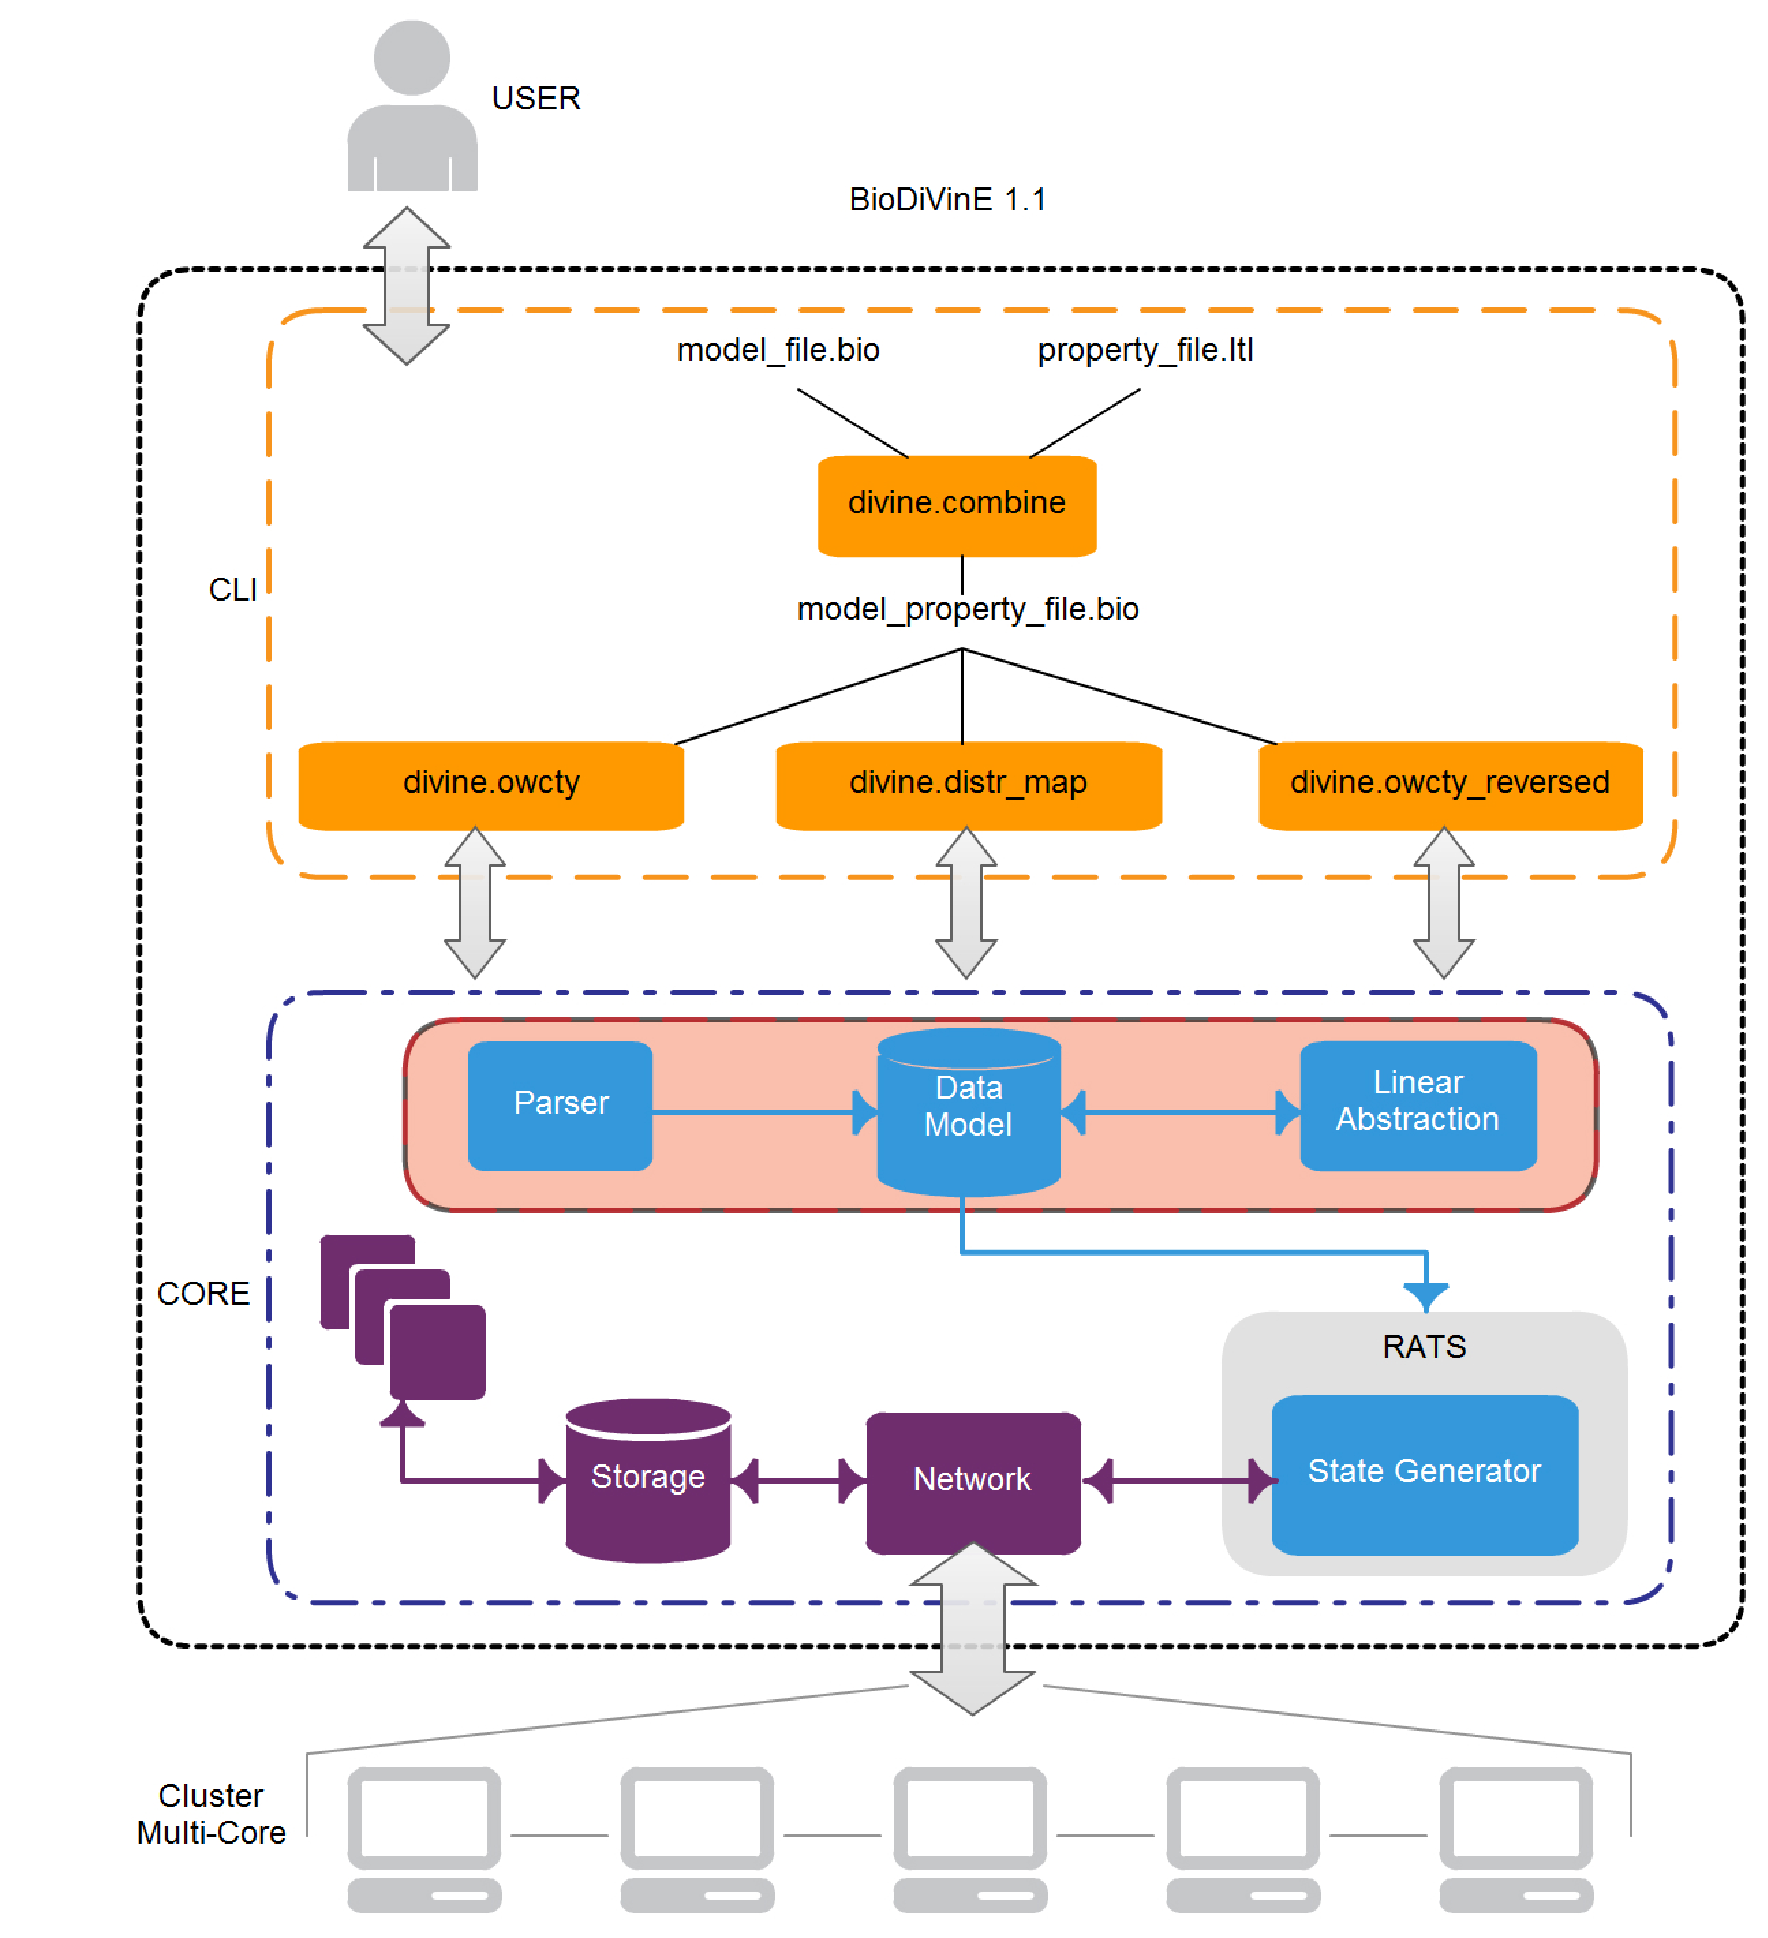
\includegraphics[width=1\textwidth]{BiodivineArchitecture2.pdf}
\caption{Diagram architekt\'ury n\'astroja BioDiVinE 1.1. V \v cervenej oblasti je zhrnut\'y n\'a\v s pr\'inos}
\end{figure}

%-------------------------------------------------------------------------------------------
\section{Vstupn\'y s\'ubor s modelom}
Hlavnou n\'apl\v nou tejto podkapitoly je zozn\'ami\v t bli\v z\v sie u\v z\'ivate\v la so syn\-taxou vstupn\'eho modelu. T\'ym sa mysl\'i s\'ubor s pr\'iponou
.bio a vyzer\'a nasledovne:
%Syntax s\'uboru s modelom vyzer\'a nasledovne:
\begin{itemize}
\item VARS : \ \textit{premenn\'a1{\bf,} premenn\'a2{\bf,} \dots{}}
\item CONSTS : \ \textit{kon\v stanta1{\bf,} hodnota1{\bf;} kon\v stanta2{\bf,} hodnota2 {\bf;} \dots{}}
\item EQ : \ \textit{premenn\'a1 = rovnica1}
\item EQ : \ \textit{premenn\'a2 = rovnica2}
\item THRES : \ \textit{premenn\'a1{\bf:} prah1{\bf,} prah2{\bf,} prah3{\bf,} \dots{}}
\item THRES : \ \textit{premenn\'a2{\bf:} prah1{\bf,} prah2{\bf,} \dots{}}
\item VAR\_POINTS : \ \textit{premenn\'a1{\bf:} po\v cet\_bodov{\bf,} po\v cet\_segmentov{\bf;} premenn\'a2{\bf:} po\v cet\_bodov{\bf,} po\v cet\_segmentov}
\item INIT : \ \textit{premenn\'a1{\bf:} od{\bf,} do{\bf;} premenn\'a2{\bf:} od{\bf,} do}
\item system async;
\end{itemize}
Nieko\v lko vysvetliviek a obmedzen\'i:
\begin{enumerate}
\item V\v setko, \v co je p\'isan\'e neskosen\'ym p\'ismom, mus\'i zosta\v t zachovan\'e. Naopak to, \v co je nap\'isan\'e skosen\'ym p\'ismom, treba 
nahradi\v t vlastn\'ymi hodnotami.
\item Biele znaky s\'u kompletne ignorovan\'e, d\^ ole\v zit\'e s\'u iba odde\v lova\v ce vyzna\v cen\'e hrub\'ym p\'ismom (: ; , =). Na koncoch riadkov sa 
nikdy odde\v lova\v c nesmie nach\'adza\v t s v\'ynimkou posledn\'eho riadku (system async;).
\item N\'azvy premenn\'ych a kon\v st\'ant musia ako prv\'y znak obsahova\v t p\'ismeno nasledovan\'e \v lubovolnou kombin\'aciou p\'ismen, \v c\'isel a 
znakov \_\ \textasciitilde{}\ \{\ \}.
\item \v C\'isla maj\'u tvar cel\'ych alebo desatinn\'ych \v c\'isel s desatinnou bodkou.
\item Riadok (CONSTS) nie je povinn\'y. Je tie\v z mo\v zn\'e pou\v z\'iva\v t iba nepomenovan\'e kon\v stanty (\v ci\v ze \v c\'isla).
\item Riadky (VARS) a (CONSTS) sa musia nach\'adza\v t pred ostatn\'ymi riadkami -- s\'u \'uvodn\'e.
\item Riadok (VAR\_POINTS) nie je povinn\'y a \textit{po\v cet\_bodov} znamen\'a po\v cet bodov, v ktor\'ych bud\'u evaluovan\'e regula\v cn\'e funkcie 
pre dan\'u premenn\'u, a {\it po\v cet\_segmentov} ur\v cuje po\v cet r\'amp, na ktor\'e sa tieto funkcie preved\'u.
\item Hodnoty {\it od} a {\it do} v riadku (INIT) musia by\v t niektor\'e z hodn\^ ot v pr\'islu\v snom riadku (THRES) pre dan\'u premenn\'u, pre ktor\'e
mus\'i plati\v t {\it od} $<$ {\it do}.
\item Ka\v zd\'a premenn\'a ma povinn\'y vlastn\'y riadok (EQ) a (THRES) a mus\'i sa nach\'adza\v t aj v riadku (INIT) s pr\'islu\v sn\'ymi hodnotami.
\item Riadok (system async;) je povinn\'y a mus\'i sa nach\'adza\v t na konci s\'uboru z historick\'ych d\^ ovodov.
\item Rovnica v riadku (EQ) je matematicky pop\'isan\'a v kapitole \ref{sec:model}.B konkr\'etne v z\'apise \ref{eq:equationDescribtion} a v be\v znom jazyku 
ni\v z\v sie:
\begin{itemize}
\item Parser podporuje un\'arnu oper\'aciu $-$, bin\'arne oper\'acie $+$, $-$ a $*$ a gu\v lat\'e z\'atvorky, ktor\'e m\^ o\v zu by\v t vnoren\'e \v lubovolne
ve\v la kr\'at.
\item Rovnica m\^ o\v ze okrem oper\'aci\'i a z\'atvoriek obsahova\v t pomenovan\'e aj nepomenovan\'e kon\v stanty, premenn\'e a nasleduj\'uce regula\v cn\'e 
funkcie (vi\v d z\'apis \ref{eq:regulatingFunctions}):
\begin{itemize}
\item rpcoor(premenn\'a, prah1, prah2, hodnota1, hodnota2), \\rmcoor(premenn\'a, prah1, prah2, hodnota1, hodnota2),
\item rp(premenn\'a, prah1, prah2, parameter1, parameter2),\\rm(premenn\'a, prah1, prah2, parameter1, parameter2),
\item hp(premenn\'a, prah, parameter1, parameter2),\\hm(premenn\'a, prah, parameter1, parameter2),
\item sp(premenn\'a, faktor, prah, parameter1, parameter2),\\sm(premenn\'a, faktor, prah, parameter1, parameter2),
\item spinv(premenn\'a, faktor, prah, parameter1, parameter2),\\sminv(premenn\'a, faktor, prah, parameter1, parameter2),
\item hillp(premenn\'a, prah, faktor, parameter1, parameter2),\\hillm(premenn\'a, prah, faktor, parameter1, parameter2),
\end{itemize}
\item \' Uvodn\'e znaky (r, h, s) m\^ o\v zu by\v t zadan\'e aj ako ve\v lk\'e p\'ismen\'a.
\item Znak (p) resp. (m) znamen\'a (+) resp. (--) v zmysle rast\'ucej resp. klesaj\'ucej funkcie.
\item Premenn\'a mus\'i by\v t jedna zo sk\^ or uveden\'ych premenn\'ych v riadku (VARS).
\item Hodnoty (prah, faktor, hodnota, parameter) m\^ o\v zu by\v t zadan\'e ako pomenovan\'e alebo nepomenovan\'e kon\v stanty.
\item Prah mus\'i by\v t jednou z prahov\'ych hodn\^ ot premennej.
\item \textbf{Nie je mo\v zn\'e n\'asobi\v t spolu rovnak\'e premenn\'e ani premenn\'u s regula\v cn\'ymi funkciami z\'avysl\'imi od tejto premennej ani
samotn\'e regula\v cn\'e funkcie z\'avysl\'e na rovnakej premennej.} Bolo by to poru\v senie pravidla o stupni premennej z kapitoly \ref{sec:model}.A.
\end{itemize}
\end{enumerate}

%-------------------------------------------------------------------------------------------
\section{Vstupn\'y s\'ubor s vlastnos\v tou}
S\'ubor s vlastnos\v tou alebo vlastnos\v tami je detailne pop\'isan\'y v pr\'aci \cite{Jaros-thesis}. Tu si iba v kr\'atkosti zhrnieme syntax. S\'ubor 
s pr\'iponou .ltl m\^ o\v ze obsahova\v t nasleduj\'uce riadky:
\begin{itemize}
\item \#define \ {\it n\'azov\_premennej \ hodnota\_premennej}
\item \#property \ {\it vlastnos\v t\_vo\_forme\_ltl\_formule}
\end{itemize}
a platia pre ne nasleduj\'uce pravidl\'a:
\begin{enumerate}
\item S\'ubor m\^ o\v ze obsahova\v t \v lubovoln\'y po\v cet defin\'ici\'i (riadok \#define), mali by sa v\v sak odli\v sova\v t v n\'azve premennej. Ten m\^ o\v ze obsahova\v t
mal\'e p\'ismen\'a, \v c\'isla a znak \_. Za\v c\'ina\v t ale musia bu\v d p\'ismenom alebo znakom \_.
\item Hodnota premennej je v podstate v\'yraz s logickou hodnotou (\v ci\v ze atomick\'a propoz\'icia, AP (vi\v d kapitolu \ref{sec:logika})). T\'a m\^ o\v ze 
ma\v t bu\v d priamo
hodnotu {\it true} alebo {\it false} alebo m\^ o\v ze by\v t tvoren\'a re\v tazcom obsahuj\'ucim meno nejakej premennej z modelu, rela\v cn\'y oper\'ator (<, >, <=, >=) a \v c\'iseln\'u 
hodnotu (cel\'u alebo re\'alnu), ktor\'a sa mus\'i nach\'adza\v t medzi prahov\'ymi hodnotami premennej z modelu.
\item Po\v cet riadkov (\#property) tie\v z nie je obmedzen\'y, ale u\v z\'ivate\v l by mal vedie\v t, \v ze ka\v zd\'y tak\'yto riadok znamen\'a nov\'u 
vlastnos\v t, ktor\'a sa bude testova\v t na modeli a to znamen\'a v\'ypo\v ctov\'u r\'e\v ziu.
\item Samotn\'a formula {\it vlastnos\v t\_vo\_forme\_ltl\_formule} m\^ o\v ze by\v t tvoren\'a nasleduj\'ucimi hodnotami:
\begin{itemize}
\item Un\'arnymi tempor\'alnymi oper\'atormi ({\bf X}$\phi$, {\bf F}$\phi$, {\bf G}$\phi$) a bin\'arnymi tempor\'alnymi oper\'atormi ($\phi${\bf R}$\psi$, 
$\phi${\bf U}$\psi$)(vi\v d kapitolu \ref{sec:logika}), kde $\phi$ a $\psi$ s\'u v\'yrazy s logickou hodnotou.
\item V\'yrazmi s logickou hodnotou, ktor\'e s\'u \v dalej tvoren\'e logick\'ymi oper\'atormi ({\bf !} -- neg\'acia, {\bf \&\&} -- konjunkcia, {\bf ||} -- 
disjunkcia, {\bf ->} -- implik\'acia, {\bf <->} -- ekvivalencia) a premenn\'ymi definovan\'ymi na za\v ciatku s\'uboru.
\item Syntax podporuje aj \v lubovolne vnoren\'e gu\v lat\'e  z\'atvorky.
\end{itemize}
\item Pre \'uplnos\v t treba doda\v t, \v ze t\'ato syntax podporuje aj p\'ar \v dals\'ich, roz\v s\'iren\'ych oper\'atorov a takmer ku ka\v zd\'emu e\v ste
druh\'y mo\v zn\'y z\'apis, ale n\'a\v s v\'ypo\v cet je dostato\v cn\'y pre z\'apis \v lubovolnej LTL formule.
\end{enumerate}

%-------------------------------------------------------------------------------------------
\section{Priebeh procesu}
Po zavolan\'i CLI spolu so zadan\'ymi vstupn\'ymi parametrami sa najsk\^ or skontroluje ich po\v cet. Ak je tento men\v s\'i, program vyp\'i\v se \textit{help}
ponuku /*odkaz na obrazok s nou*/. V opa\v cnom pr\'ipade skontroluje existenciu vstupn\'ych s\'uborov a pred\'a ich pomocn\'emu n\'astroju {\it divine.combine}.
Ten zist\'i po\v cet vlastnost\'i a pre ka\v zd\'u z nich vytvor\'i nov\'y s\'ubor a z\'arove\v n prevedie vlastnos\v t z LTL formule na B\"uchiho automat. 
Tento v\'ystupn\'y s\'ubor m\'a tie\v z koncovku .bio, ale je iba pomocn\'y a pred ukon\v cen\'im CLI bude zmazan\'y. \v Dalej sa zist\'i po\v zadovan\'y 
overovac\'i algoritmus. M\^ o\v ze \'is\v t o algoritmy {\it owcty}, {\it distr\_map} alebo {\it owcty\_reversed}. \v Ziadne in\'e nie s\'u pr\'ipustn\'e.

Vybran\'y algoritmus sa spust\'i pre ka\v zd\'y novovytvoren\'y s\'ubor .bio ako n\'astroj {\it divine.n\'azov\_algoritmu} a predaj\'u sa mu pr\'ipadn\'e 
parametre. Potom sa vstup pred\'a triede s parserom a vytvor\'i sa datov\'y model, ktor\'y prejde line\'arnou aproxim\'aciou, ak je to potrebn\'e. T\'ym sa
mysl\'i pr\'ipad, ke\v d rovnice modelu obsahuj\'u aspo\v n jednu Hillovu funkciu alebo aspo\v n jednu sigmoid\'alnu funkciu. Heavisidove funkcie sa 
upravuj\'u zvl\'a\v s\v t hne\v d po na\v c\'itan\'i, preto\v ze ich mo\v zno previes\v t na jedin\'u rampu a teda line\'arna aproxim\'acia pre ne nem\'a 
zmysel. 

Prahov\'e hodnoty vygenerovan\'e aproxim\'aciou aj prevodom Heavisidov\'ych funkci\'i sa ulo\v zia medzi ostatn\'e. To na jednu stranu zvy\v suje 
v\'ypo\v ctov\'u r\'e\v ziu, preto\v ze sa zv\" a\v c\v suje stavov\'y priestor generovan\'y nasleduj\'ucou obd\'l\v znikovou aproxim\'aciou. A to line\'arne 
k po\v ctu nov\'ych prahov\'ych hodn\^ ot. No na strane druhej sa t\'ym zlep\v suje presnos\v t tejto aproxim\'acie a cel\'eho v\'ypo\v ctu, preto\v ze sa 
abstrahovan\'y model pribli\v zuje skuto\v cn\'emu spojit\'emu modelu.

U\v z spomenut\'a obd\'l\v znikov\'a aproxim\'acia vygeneruje RATS (vi\v d \ref{sec:abstraction}.B), \v ci\v ze diskr\'etny syst\'em p\^ ovodne spojit\'eho 
modelu, ktor\'y sa overuje proti vlastnosti v podobe automatu. Ak ju RATS sp\'l\v na, potom mo\v zno s istotou tvrdi\v t, \v ze aj p\^ ovodn\'y model t\'uto
vlastnos\v t sp\'l\v na. Naopak, ak je vygenerovan\'y protipr\'iklad, tento v\^ obec nemus\'i zodpoveda\v t protipr\'ikladu v skuto\v cnom spojitom modeli.
Av\v sak st\'ale plat\'i, \v ze model, \v ci u\v z abstrahovan\'y alebo skuto\v cn\'y dan\'u vlastnos\v t nesp\'l\v na. \cite{BIODIVINE}
/*dalo by sa este spomenut, ze owcty a owcty\_reversed dokazu skumat aj samostatne reachabilitu*/

%-------------------------------------------------------------------------------------------
\chapter{Implement\' acia}
/*asi by sa hodilo napisat v com som pisal parser a scanner a jake su tam subory, dalej popisat triedy datoveho modelu a CLI*/

\section{Parser}
Na \'uvod je treba poveda\v t, \v ze za v\'yrazom parser sa ukr\'yva aj druh\'y pomocn\'y n\'astroj tzv. scanner. Samotn\'y parser je n\'astroj na syntaktick\'u 
anal\'yzu vstupu a v niektor\'ych jednoduch\'ych pr\'ikladoch m\^ o\v ze by\v t dostato\v cn\'y, ale nie v na\v som. Aby bolo parsovanie \'uspe\v sn\'e mus\'i
mu predch\'adza\v t e\v ste lexik\'alna anal\'yza a t\'u m\'a na starosti pr\'ave scanner, ktor\'y zjednodu\v sene povedan\'e na\v c\'itava "slov\'a". Tie potom
posiela parseru, ktor\'y z nich sklad\'a "vety", respekt\'ive vzory. Akon\'ahle je nejak\'y vzor rozpoznan\'y, in\v strukcie parseru povedia, ak\'u akciu
m\'a s d\'atami vykona\v t.

Pre vytvorenie parseru a scanneru s\'u k dispoz\'icii sestersk\'e programy. Najstar\v sie z nich s\'u {\it flex} a {\it bison}. Tie sa v\v sak uk\'azali by\v t
a\v z pr\'ili\v s zastaran\'e a neschopn\'e vytvori\v t jednoduch\'u \v strukt\'uru typu trieda, ktor\'a by sa dala \v lahko za\v cleni\v t do u\v z 
existuj\'uceho k\'odu. \v Dal\v sou mo\v znos\v tou, ktor\'u sme zva\v zovali, boli programy {\it flex++} a {\it bison++}. Tie \'udajne podporuj\'u triedy, 
ale n\'ajs\v t k nim pou\v zite\v ln\'y u\v z\'ivate\v lsk\'y manu\'al sa uk\'azalo by\v t nemo\v zn\'e. Naopak programy {\it flexc++} \cite{flexc++} a 
{\it bisonc++} \cite{bisonc++} s\'u preh\v ladne zdokumentovan\'e a ve\v lmi dobre za\v clenite\v ln\'e do zdrojov\'eho k\'odu v jazyku c++, preto sa 
uk\'azali by\v t tou najlep\v sou vo\v lbou.
/*mozno opisat este detailnejsie subory ktorych a to tyka a co priblizne obsahuju*/

\section{D\'atov\'y model}

\section{Konzolov\'e u\v z\'ivate\v lsk\'e prostredie CLI}

%-------------------------------------------------------------------------------------------
\chapter{Pou\v zitie programu}

%-------------------------------------------------------------------------------------------
\chapter{Case study}

%-------------------------------------------------------------------------------------------
\chapter{Z\' aver}


\bibliographystyle{plain} 
\bibliography{dp1}

\chapter*{Pr\' iloha}


\end{document}
